\chapter{Optimising Towards Unlikelihood: Data-Divergent Fine-Tuning of Generative Neural Networks}
\label{ch:divergent}

This chapter details experiments in the divergent fine-tuning of pre-trained models with the goal of diverging from the likelihood-driven data modelling approach, towards the generation of novel, unseen data distributions.
The work in this chapter was first published in the paper \textit{'Amplifying The Uncanny'} was published at the 8th Conference on Computation, Communication, Aesthetics \& X (xCoAx) \citep{broad2020amplifying}. 
These experiments were the first peer-reviewed and published attempt at divergent fine-tuning that does not rely on imitation based learning. Other approaches to divergent fine-tuning are detailed in \S \ref{survey:divergent}. 
It should be noted that the results presented here are not the exact results first shared in \cite{broad2020amplifying}. The experiments were re-run, so that more data could be logged, and more variations of parameter settings and loss functions could be compared.

\section{Motivation}
\label{c4:sec:motivation}

Following the work presented in Chapter \ref{ch:unstable_eq}, I was motivated to explore further the possibility of training generative neural networks without data. 
However, given the rather idiosyncratic nature of the arrangements of neural networks and loss functions presented in the last chapter, I wanted to pursue an approach that was more deliberate, with experiments that could be repeated by others more easily. 

Instead of training neural networks completely from random initialisation, I wanted to find new ways to fine-tune pre-trained models using novel loss functions and auxiliary networks. 
The reasoning for this was that it was clear, based on experiments such as deepdream \citep{mordvintsev2015inceptionism} and Tom White's perception engines \citep{white2018perception,white2019shared} show that CNN-based computer vision models had powerful representations baked into them, and that these representations could be utilised in the context of fine-tuning models to reveal otherwise hidden aspects of machine vision.
My intuition was that if pre-trained image recognition models could be used for generating individual images, then they could also be used for fine-tuning existing generative models, in a data-divergent fashion.

The computational resources required to train the then state-of-the-art models such as BigGAN \citep{brock2018large} and StyleGAN \citep{karras2019style}  were prohibitive in the context of this research. 
However, transfer learning and fine tuning was something that I could experiment much more rapidly in divergent ways. 
This has become increasingly common amongst creative practitioners working with high fidelity models \citep{berns2020bridging}. 
Instead of training from scratch, fine-tuning pre-trained models to be fine-tuned in divergent ways was something that I could experiment much more rapidly. 

\section{Method}
\label{c4:sec:method}

These experimentswere performed using pre-trained checkpoints from the original StyleGAN, which had been trained on the FFHQ dataset \citep{karras2019style}. 
Three different checkpoints were used: one at 256x256 resolution, one at 512x512 resolution, and one at 1024x1024 resolution. 
These different checkpoints were available because the original StyleGAN implemented the progressive growing training method in \citep{karras2017progressive}.
The checkpoints used were not the official StyleGAN models released by NVIDIA, but instead, a PyTorch reimplementation \citep{rosinality2019style}.
This alternative implementation was used because  the checkpoints contained both the weights of the generator and the discriminator.\footnote{The NVIDIA official releases of StyleGAN weights only have the checkpoints of the generator, not the discriminator.}.

The standard GAN training objective is:

\begin{equation} 
\min_{G}\max_{D}\mathbb{E}_{x\sim p_{\text{data}}(x)}[\log{D(x)}] +  \mathbb{E}_{z\sim p_{\text{z}}(z)}[1 - \log{D(G(z))}]
\end{equation}

Where the generator network $G$ is trying to minimise the likelihood of its generated samples being classified as fake, whereas the discriminator is optimised to maximise classification accuracy between real data samples and fake (generated) samples.
The modification in this training regime is to invert this loss function following training, and then instead optimise the generator toward maximising the likelihood that its generated samples are correctly classified as being fake:

\begin{equation} 
  \max_{G}\mathbb{E}_{x\sim p_{\text{data}}(x)}[\log{D(x)}] +  \mathbb{E}_{z\sim p_{\text{z}}(z)}[1 - \log{D(G(z))}]
  \label{eq:inverted-adv-loss}
  \end{equation}

In this procedure, there is no training objective for the discriminator. 
The weights of the discriminator are kept frozen, and the network is simply used to calculate the loss function for the generator.
Figure \ref{fig:c4:gan-diagrams} shows visually the difference between the standard GAN training regime and this modified fine-tuning procedure. 

\begin{figure}[!htbp]
  \centering
  \subfloat[]{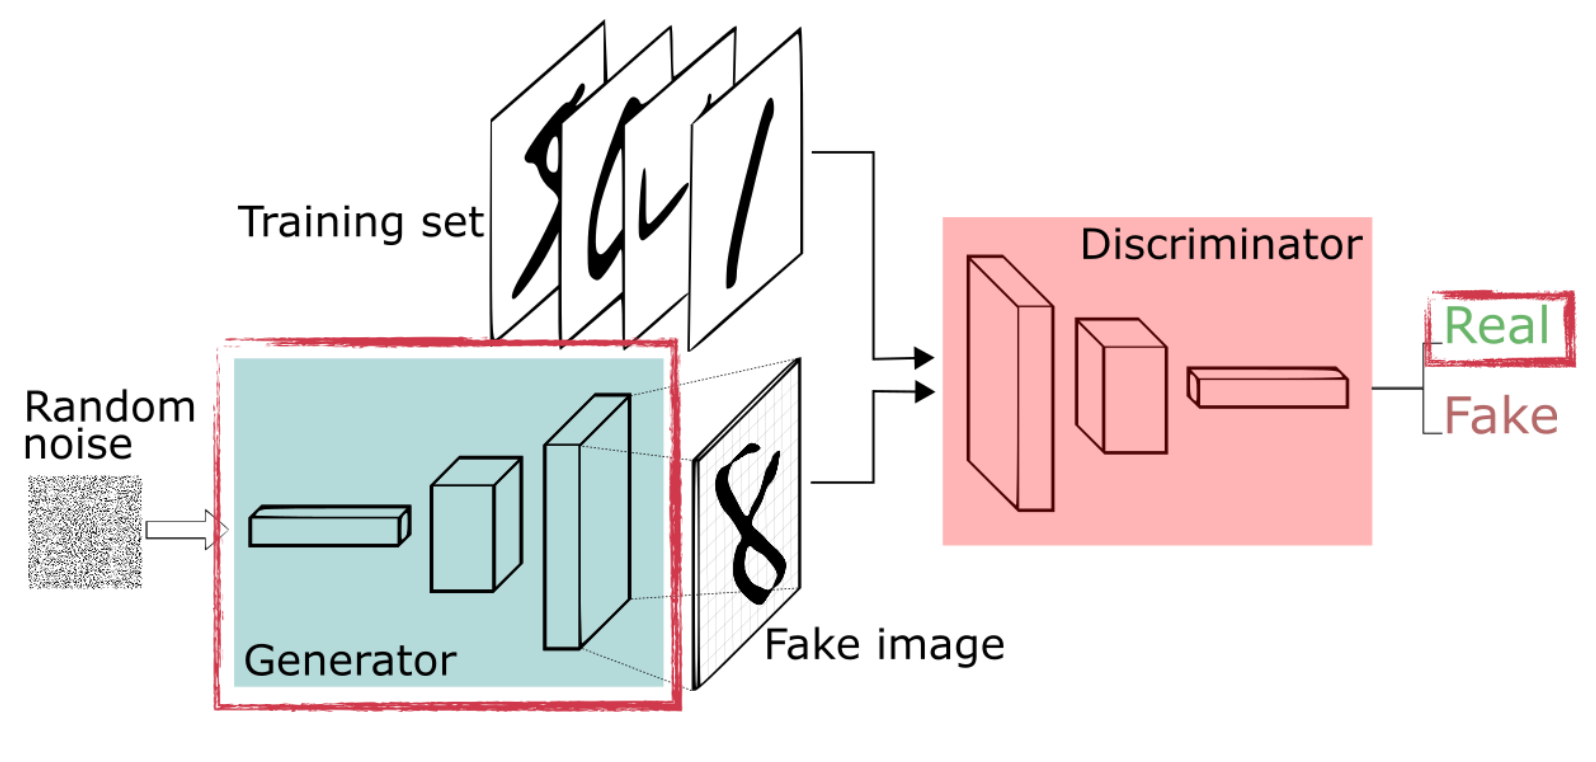
\includegraphics[width=1\textwidth]{figures/c4_divergent/diagrams/normal-gan-training.png}}
  \hfill
  \subfloat[]{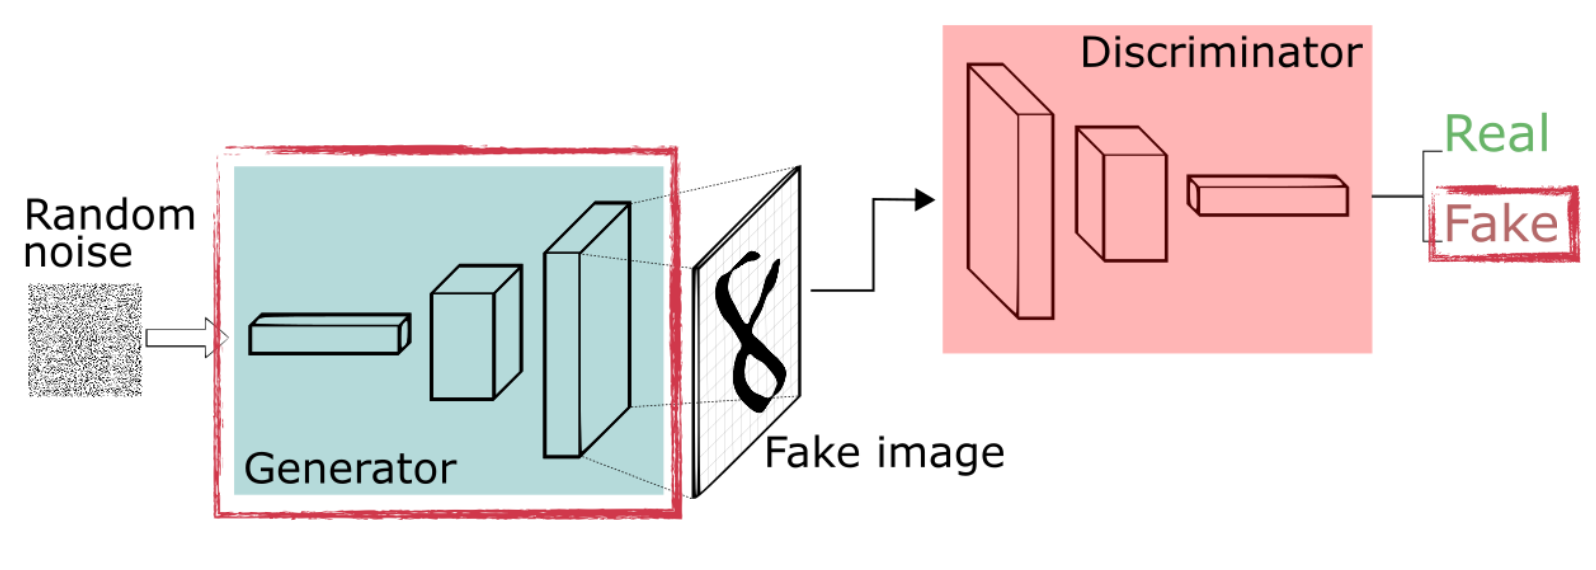
\includegraphics[width=1\textwidth]{figures/c4_divergent/diagrams/inverted-gan-loss.png}}
  \caption[Adversarial and inverted adversarial loss diagram]{Diagrams showing the standard GAN training regime with the loss that the generator is optimised towards (a), and the inverted adversarial loss fine-tuning procedure with the alternative loss for the generator network (b).}
  \label{fig:c4:gan-diagrams}
\end{figure}

In a second set of experiments this loss is modified to take the natural logarithm of the modified GAN loss:

\begin{equation} 
  \max_{G}\log(\mathbb{E}_{x\sim p_{\text{data}}(x)}[\log{D(x)}] +  \mathbb{E}_{z\sim p_{\text{z}}(z)}[1 - \log{D(G(z))}])
  \label{eq:ln-inverted-adv-loss}
  \end{equation}

The results from this operation can be seen in \S \ref{c4:sec:log-loss}.

For each model checkpoint (256,512 \& 1024) and loss function (inverse adversarial, log-inverse adversarial), three fine-tuning runs were performed with different parameters for batch size during training: 2, 4 \& 8.
Experimenting with different conditions for batch size was undertaken in order to determine if this would have an impact on the generated results, as it is widely assumed that increasing the batch size improves visual fidelity in the standard GAN training regime. 
My intuition was that adjusting the batch size may also impact the diversity of generated outputs.

\textbf{REWRITE FOLLOWING PARAGRAPH:}

For the standard inverted adversarial loss function (Eq. \ref{eq:inverted-adv-loss}), the fine-tuning procedure is run for 1000 iterations.
For the natural logarithm of the inverted adversarial loss function (Eq. \ref{eq:ln-inverted-adv-loss}), fine-tuning is run for 10000 iterations.
The reason for the difference in iteration count is that the log-loss is less aggressive and therefore the fine-tuning procedure does not collapse as quickly as the standard loss \ref{eq:inverted-adv-loss}.

\section{Results}
\label{c4:sec:results}

This section shows the results of the fine-tuning training procedure. 
It is divided into two sub-sections.
The first (\S \ref{c4:sec:og-loss}) shows the results of the standard inverted adversarial loss (Eq. \ref{eq:inverted-adv-loss}).
The second (\S \ref{c4:sec:log-loss}) shows the results for the natural logarithm of the inverted adversarial loss (Eq. \ref{eq:ln-inverted-adv-loss}).

\subsection{Inverted Adversarial Loss}
\FloatBarrier

This section shows the results of the standard inverted adversarial loss (Eq. \ref{eq:inverted-adv-loss}). For all of these experiments with this loss function the fine-tuning procedure was performed for 1000 iterations.
Figures \ref{fig:c4:256-OG-samples} \& \ref{fig:c4:256-OG-losses} show the generated samples and losses during fine-tuning for the 256x256 checkpoint.
Figures \ref{fig:c4:512-OG-samples} \& \ref{fig:c4:512-OG-losses} show the generated samples and losses during fine-tuning for the 512x512 checkpoint.
Figures \ref{fig:c4:1024-OG-samples} \& \ref{fig:c4:1024-OG-losses} show the generated samples and losses during fine-tuning for the 1024x1024 checkpoint.

\label{c4:sec:og-loss}
\begin{figure}[!htbp]
    \centering
    \subfloat[]{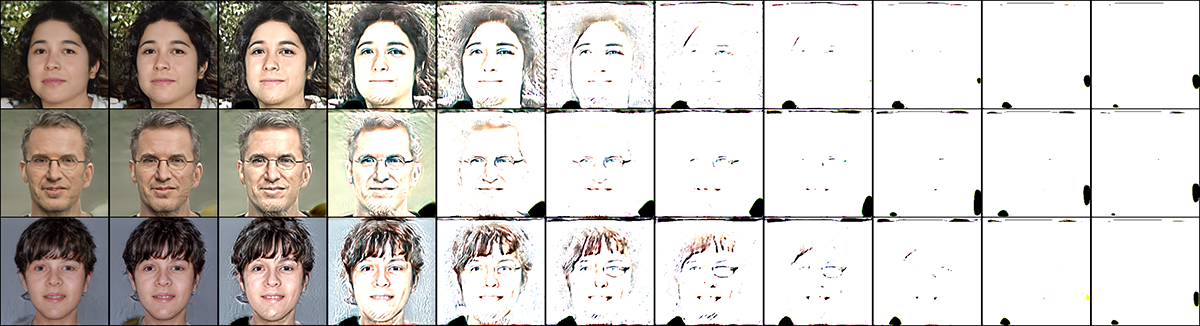
\includegraphics[width=1\textwidth]{figures/c4_divergent/gen-plots/OG/256/256-OG-2-Images-1000.png}}
    \hfill
    \subfloat[]{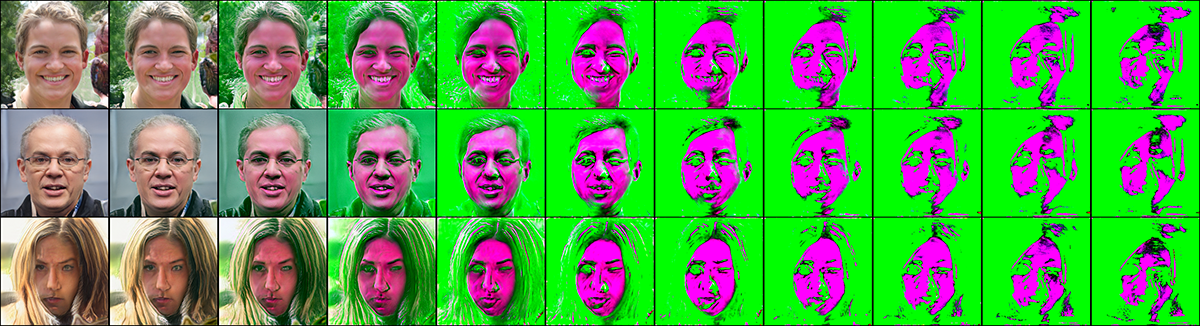
\includegraphics[width=1\textwidth]{figures/c4_divergent/gen-plots/OG/256/256-OG-4-Images-1000.png}}
    \hfill
    \subfloat[]{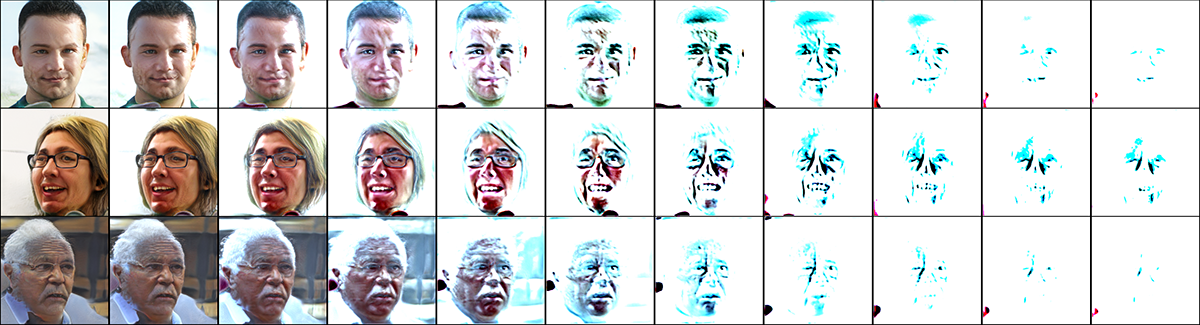
\includegraphics[width=1\textwidth]{figures/c4_divergent/gen-plots/OG/256/256-OG-8-Images-1000.png}}
    \caption[Samples of generations during the fine-tuning procedure for 256x256 StyleGAN model with the inverted adversarial loss function]{Samples of generations during the fine-tuning procedure for 256x256 StyleGAN model with the inverted adversarial loss function, at increments of 100, between training step 0-10000. (a) Results with batch size 2. (b) Results with batch size 4. (c) Results with batch size 8.}
    \label{fig:c4:256-OG-samples}
  \end{figure}

  \begin{figure}[!htbp]
    \centering
    \subfloat[]{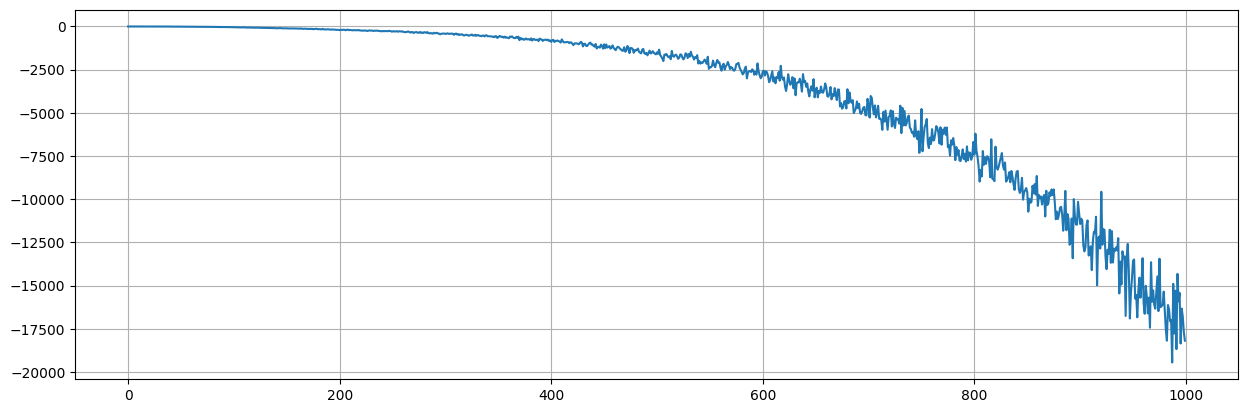
\includegraphics[width=0.8\textwidth]{figures/c4_divergent/loss-plots/OG/256/256-B2.png}}
    \hfill
    \subfloat[]{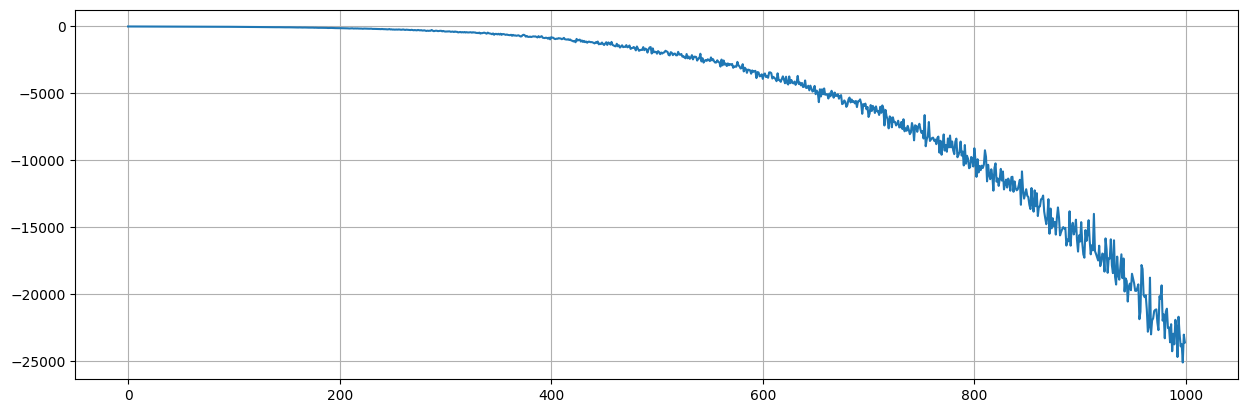
\includegraphics[width=0.8\textwidth]{figures/c4_divergent/loss-plots/OG/256/256-B4.png}}
    \hfill
    \subfloat[]{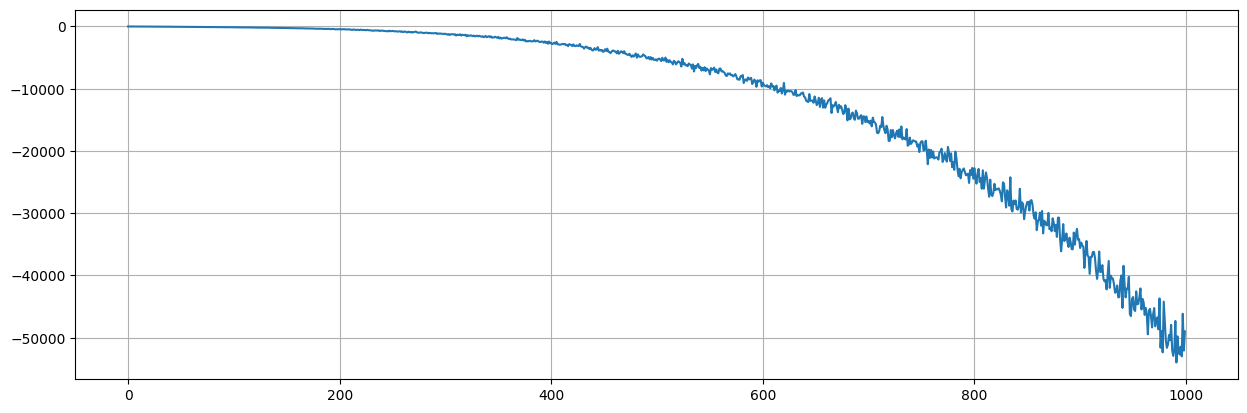
\includegraphics[width=0.8\textwidth]{figures/c4_divergent/loss-plots/OG/256/256-B8.png}}
    \caption[Loss plots for the fine-tuning procedure for 256x256 StyleGAN model with the inverted adversarial loss function]{Loss plots for the fine-tuning procedure for 256x256 StyleGAN model with the inverted adversarial loss function. (a) Results with batch size 2. (b) Results with batch size 4. (c) Results with batch size 8.}
    \label{fig:c4:256-OG-losses}
  \end{figure}

  \begin{figure}[!htbp]
    \centering
    \subfloat[]{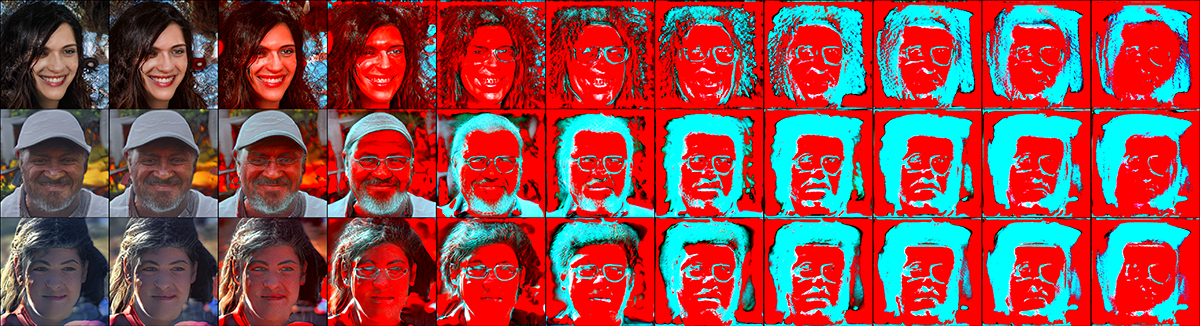
\includegraphics[width=1\textwidth]{figures/c4_divergent/gen-plots/OG/512/512-OG-2-Images-1000.png}}
    \hfill
    \subfloat[]{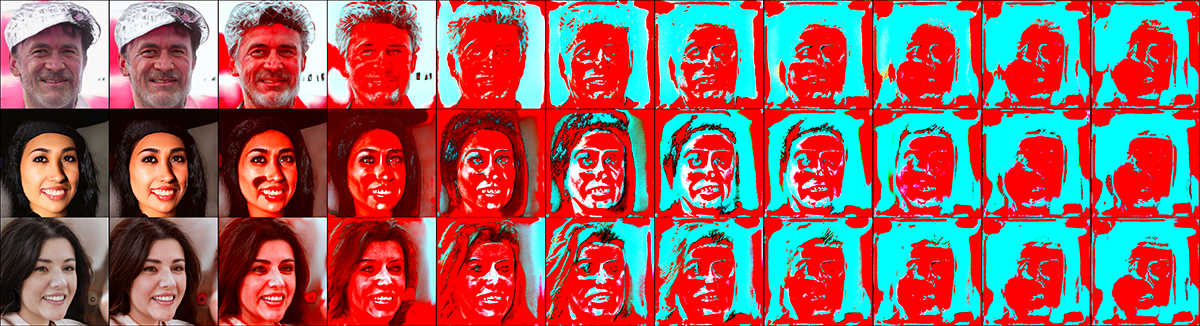
\includegraphics[width=1\textwidth]{figures/c4_divergent/gen-plots/OG/512/512-OG-4-Images-1000.png}}
    \hfill
    \subfloat[]{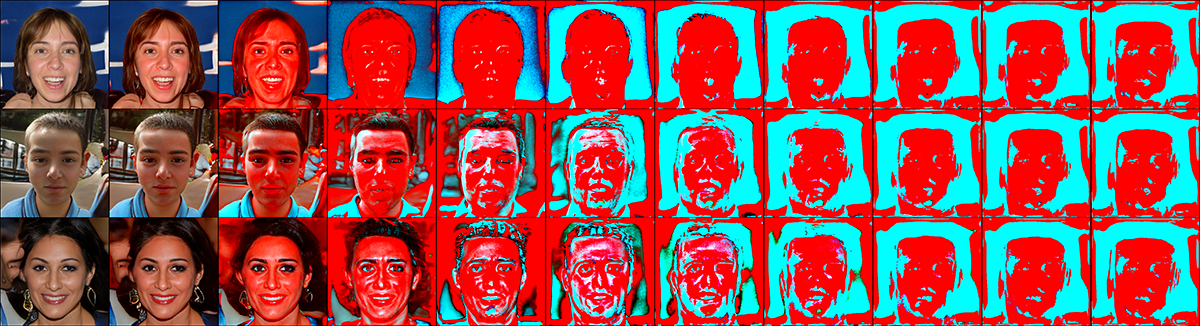
\includegraphics[width=1\textwidth]{figures/c4_divergent/gen-plots/OG/512/512-OG-8-Images-1000.png}}
    \caption[Samples of generations during the fine-tuning procedure for 512x512 StyleGAN model with the inverted adversarial loss function]{Samples of generations during the fine-tuning procedure for 512x512 StyleGAN model with the inverted adversarial loss function, at increments of 100, between training step 0-1000. (a) Results with batch size 2. (b) Results with batch size 4. (c) Results with batch size 8.}
    \label{fig:c4:512-OG-samples}
  \end{figure}

  \begin{figure}[!htbp]
    \centering
    \subfloat[]{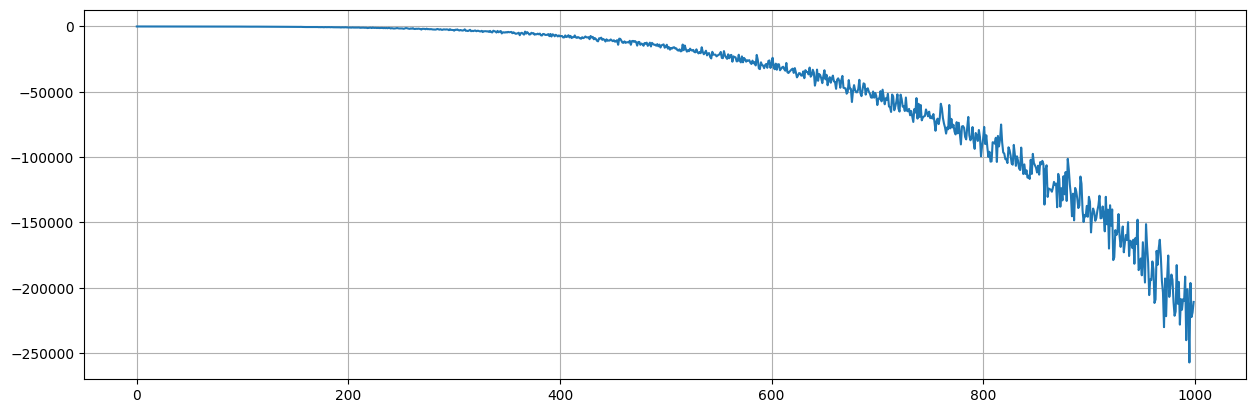
\includegraphics[width=0.8\textwidth]{figures/c4_divergent/loss-plots/OG/512/512-B2.png}}
    \hfill
    \subfloat[]{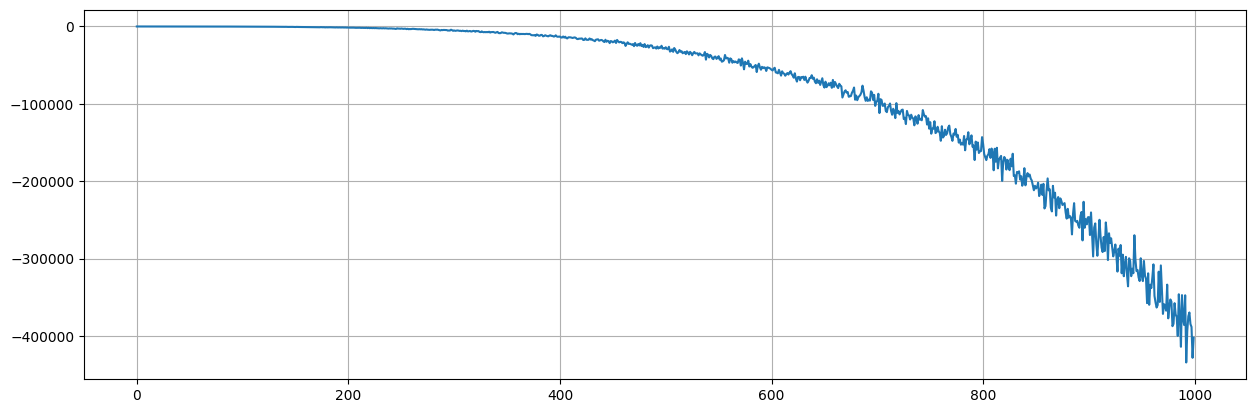
\includegraphics[width=0.8\textwidth]{figures/c4_divergent/loss-plots/OG/512/512-B4.png}}
    \hfill
    \subfloat[]{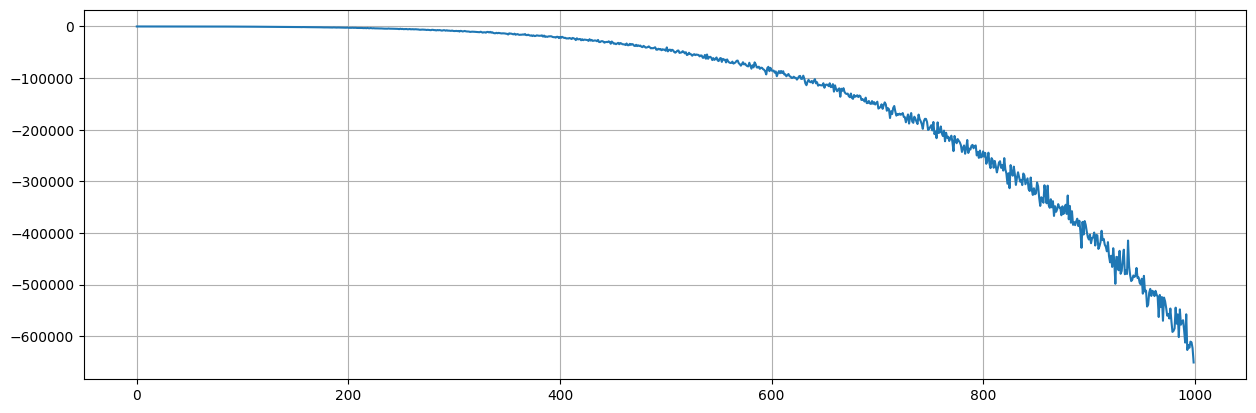
\includegraphics[width=0.8\textwidth]{figures/c4_divergent/loss-plots/OG/512/512-B8.png}}
    \caption[Loss plots for the fine-tuning procedure for 512x512 StyleGAN model with the inverted adversarial loss function]{Loss plots for the fine-tuning procedure for 512x512 StyleGAN model with the inverted adversarial loss function. (a) Results with batch size 2. (b) Results with batch size 4. (c) Results with batch size 8.}
    \label{fig:c4:512-OG-losses}
  \end{figure}

  \begin{figure}[!htbp]
    \centering
    \subfloat[]{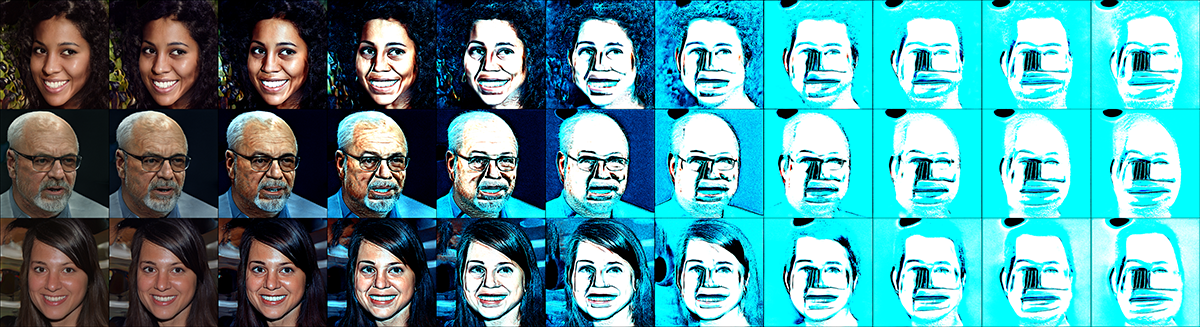
\includegraphics[width=1\textwidth]{figures/c4_divergent/gen-plots/OG/1024/1024-OG-2-Images-1000.png}}
    \hfill
    \subfloat[]{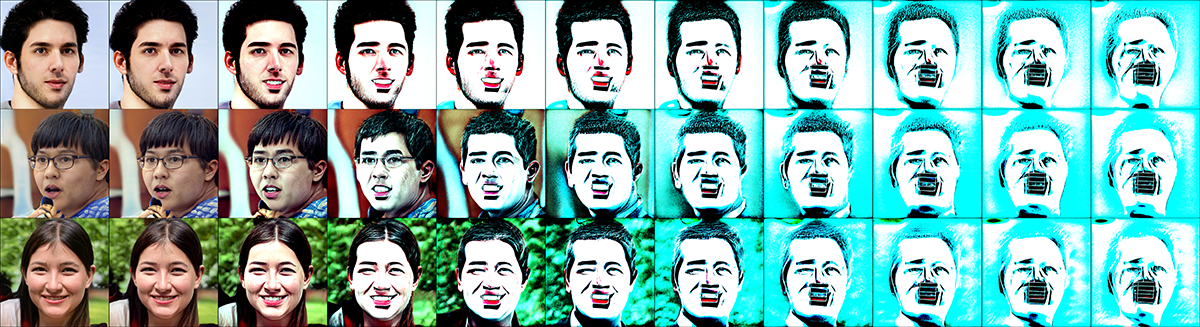
\includegraphics[width=1\textwidth]{figures/c4_divergent/gen-plots/OG/1024/1024-OG-4-Images-1000.png}}
    \hfill
    \subfloat[]{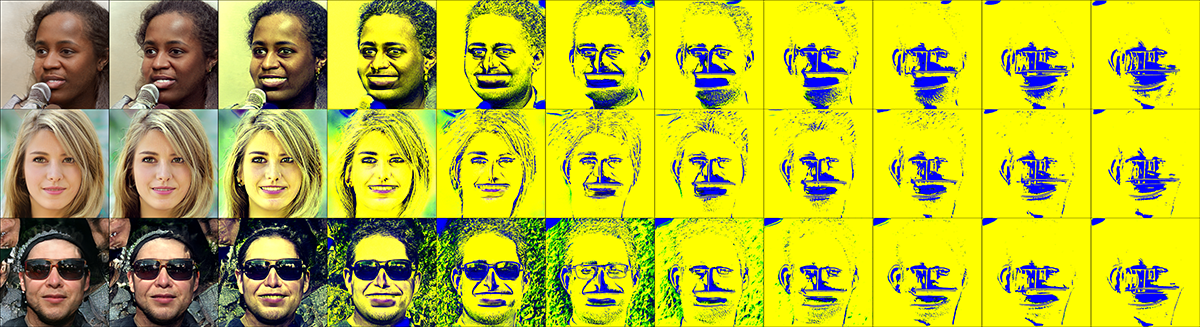
\includegraphics[width=1\textwidth]{figures/c4_divergent/gen-plots/OG/1024/1024-OG-8-Images-1000.png}}
    \caption[Samples of generations during the fine-tuning procedure for 1024x1024 StyleGAN model with the inverted adversarial loss function]{Samples of generations during the fine-tuning procedure for 1024x1024 StyleGAN model with the inverted adversarial loss function, at increments of 100, between training step 0-1000. (a) Results with batch size 2. (b) Results with batch size 4. (c) Results with batch size 8.}
    \label{fig:c4:1024-OG-samples}
  \end{figure}

  \begin{figure}[!htbp]
    \centering
    \subfloat[]{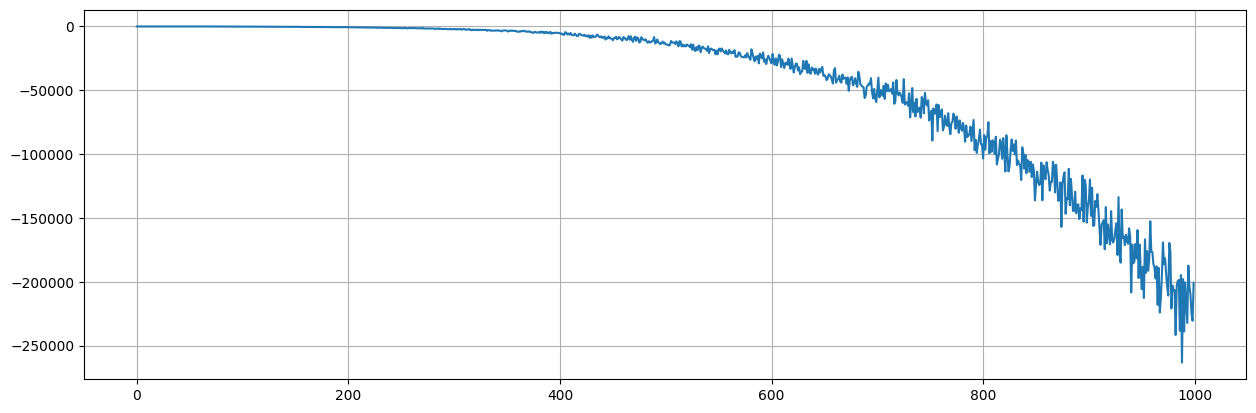
\includegraphics[width=0.8\textwidth]{figures/c4_divergent/loss-plots/OG/1024/1024-B2.png}}
    \hfill
    \subfloat[]{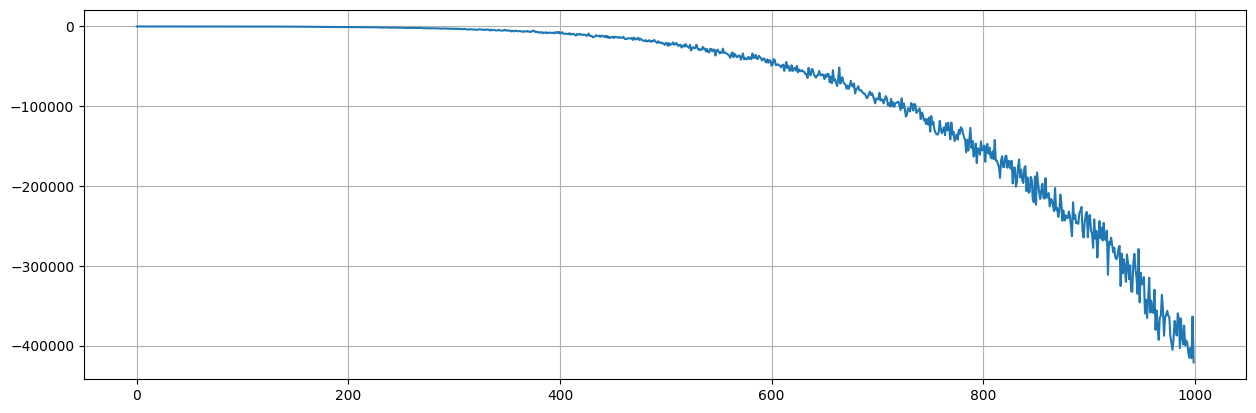
\includegraphics[width=0.8\textwidth]{figures/c4_divergent/loss-plots/OG/1024/1024-B4.png}}
    \hfill
    \subfloat[]{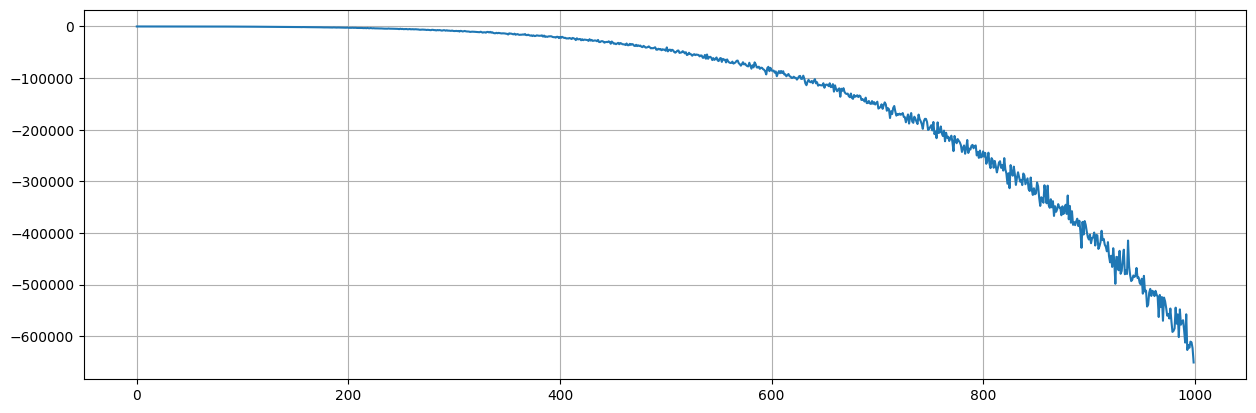
\includegraphics[width=0.8\textwidth]{figures/c4_divergent/loss-plots/OG/1024/1024-B8.png}}
    \caption[Loss plots for the fine-tuning procedure for 1024x1024 StyleGAN model with the inverted adversarial loss function]{Loss plots for the fine-tuning procedure for 1024x1024 StyleGAN model with the inverted adversarial loss function. (a) Results with batch size 2. (b) Results with batch size 4. (c) Results with batch size 8.}
    \label{fig:c4:1024-OG-losses}
  \end{figure}

\FloatBarrier

\subsection{Natural Logarithm of Inverted Adversarial Loss}
\label{c4:sec:log-loss}

This section shows the results of the standard inverted adversarial loss (Eq. \ref{eq:ln-inverted-adv-loss}). For all of these experiments with this loss function the fine-tuning procedure was performed for 10000 iterations.
Figures \ref{fig:c4:256-LOG-samples} \& \ref{fig:c4:256-LOG-losses} show the generated samples and losses during fine-tuning for the 256x256 checkpoint.
Figures \ref{fig:c4:512-LOG-samples} \& \ref{fig:c4:512-LOG-losses} show the generated samples and losses during fine-tuning for the 512x512 checkpoint.
Figures \ref{fig:c4:1024-LOG-samples} \& \ref{fig:c4:1024-LOG-losses} show the generated samples and losses during fine-tuning for the 1024x1024 checkpoint.

\begin{figure}[!htbp]
    \centering
    \subfloat[]{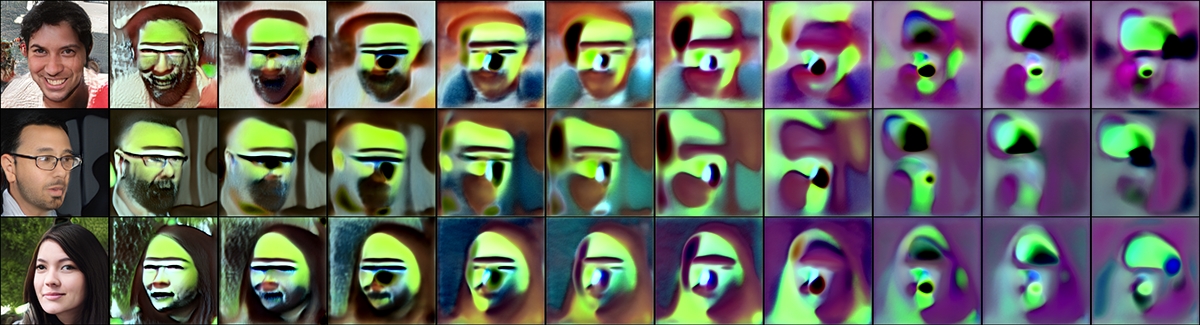
\includegraphics[width=1\textwidth]{figures/c4_divergent/gen-plots/LOG/256/256-LOG-2-Images-10000.png}}
    \hfill
    \subfloat[]{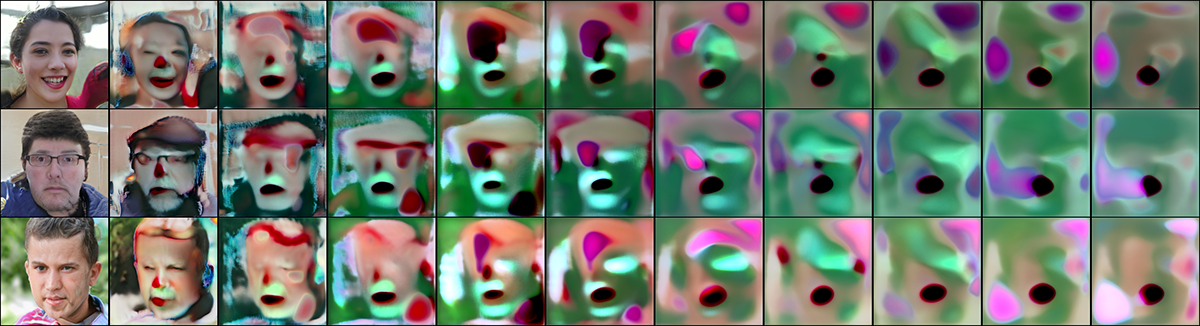
\includegraphics[width=1\textwidth]{figures/c4_divergent/gen-plots/LOG/256/256-LOG-4-Images-10000.png}}
    \hfill
    \subfloat[]{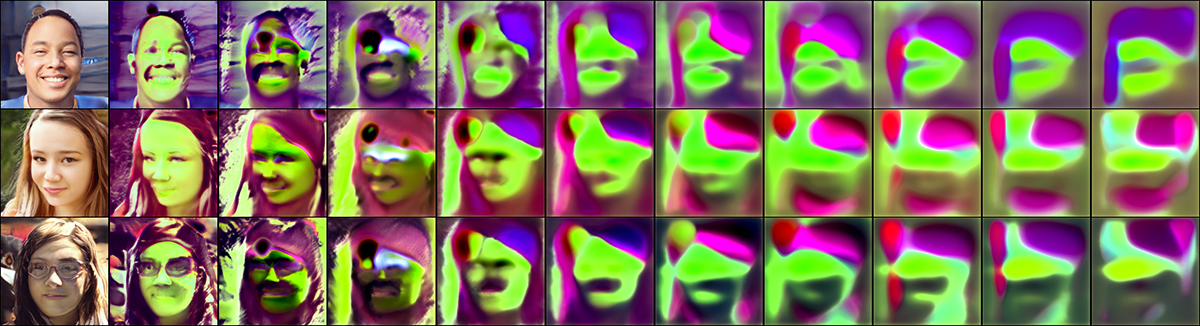
\includegraphics[width=1\textwidth]{figures/c4_divergent/gen-plots/LOG/256/256-LOG-8-Images-10000.png}}
    \caption[Samples of generations during the fine-tuning procedure for 256x256 StyleGAN model with the natural logarithm of the inverted adversarial loss function]{Samples of generations during the fine-tuning procedure for 256x256 StyleGAN model with the natural logarithm of the inverted adversarial loss function, at increments of 1000, between training step 0-10000. (a) Results with batch size 2. (b) Results with batch size 4. (c) Results with batch size 8.}
    \label{fig:c4:256-LOG-samples}
  \end{figure}

  \begin{figure}[!htbp]
    \centering
    \subfloat[]{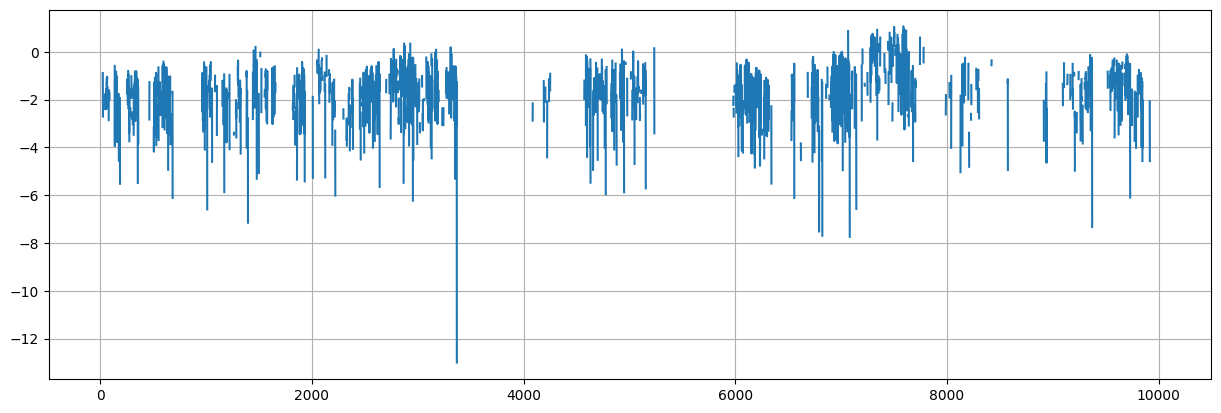
\includegraphics[width=0.8\textwidth]{figures/c4_divergent/loss-plots/LOG/256/256-B2.png}}
    \hfill
    \subfloat[]{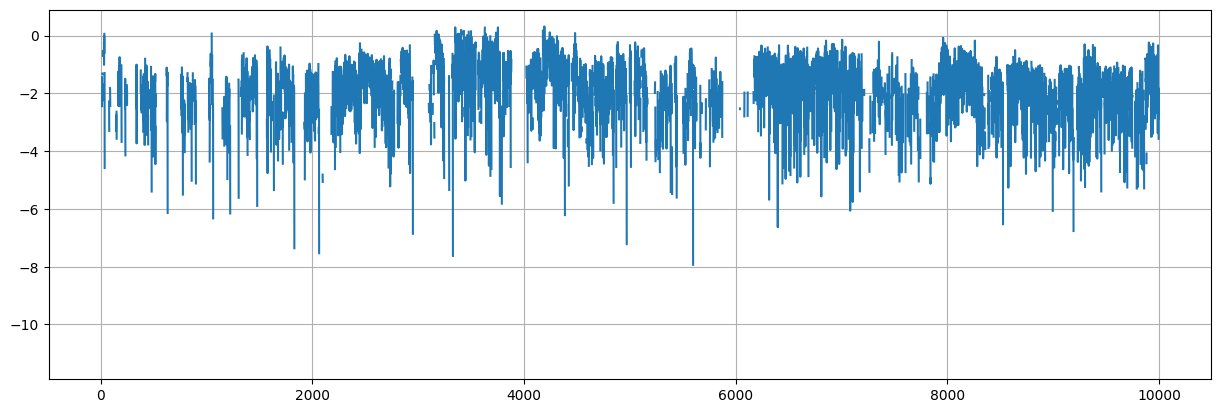
\includegraphics[width=0.8\textwidth]{figures/c4_divergent/loss-plots/LOG/256/256-B4.png}}
    \hfill
    \subfloat[]{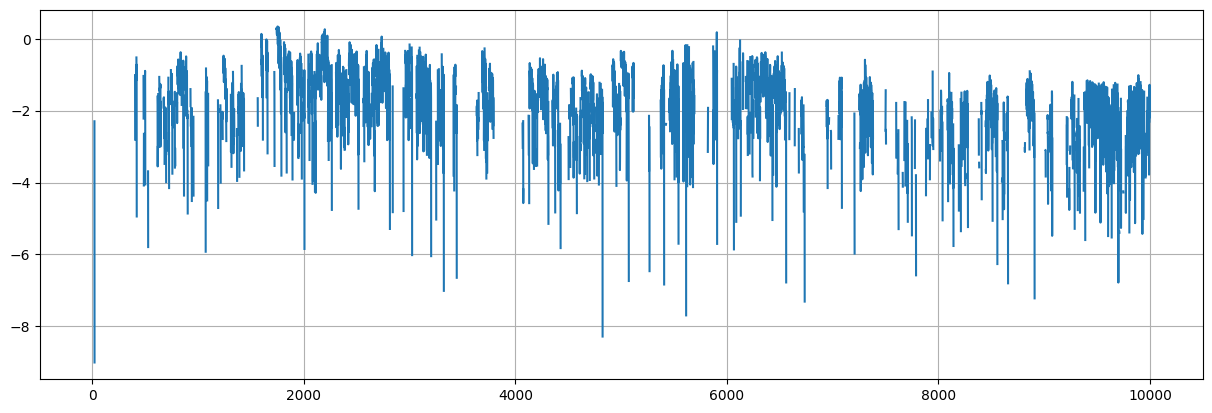
\includegraphics[width=0.8\textwidth]{figures/c4_divergent/loss-plots/LOG/256/256-B8.png}}
    \caption[Loss plots for fine-tuning procedure for 256x256 StyleGAN model with the natural logarithm of the inverted adversarial loss function]{Loss plots for fine-tuning procedure for 256x256 StyleGAN model with the natural logarithm of the inverted adversarial loss function. (a) Results with batch size 2. (b) Results with batch size 4. (c) Results with batch size 8. Note: gaps in the plot are where the loss was undefined from taking the log of a negative number.}
    \label{fig:c4:256-LOG-losses}
  \end{figure}

  \begin{figure}[!htbp]
    \centering
    \subfloat[]{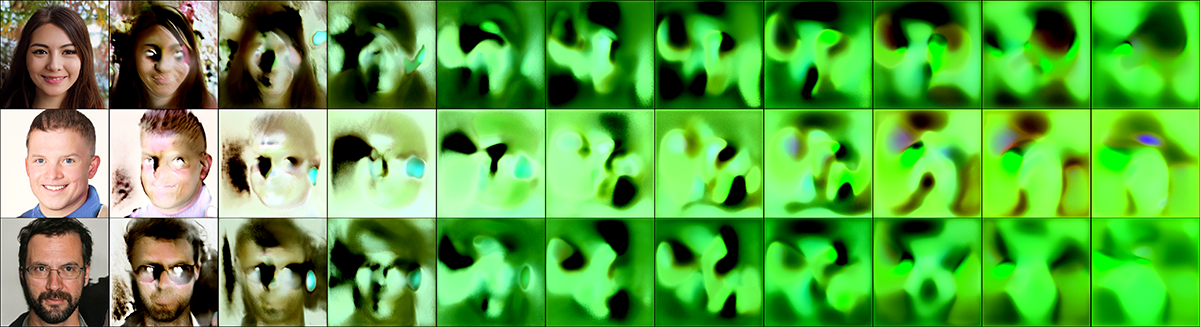
\includegraphics[width=1\textwidth]{figures/c4_divergent/gen-plots/LOG/512/512-LOG-2-Images-10000.png}}
    \hfill
    \subfloat[]{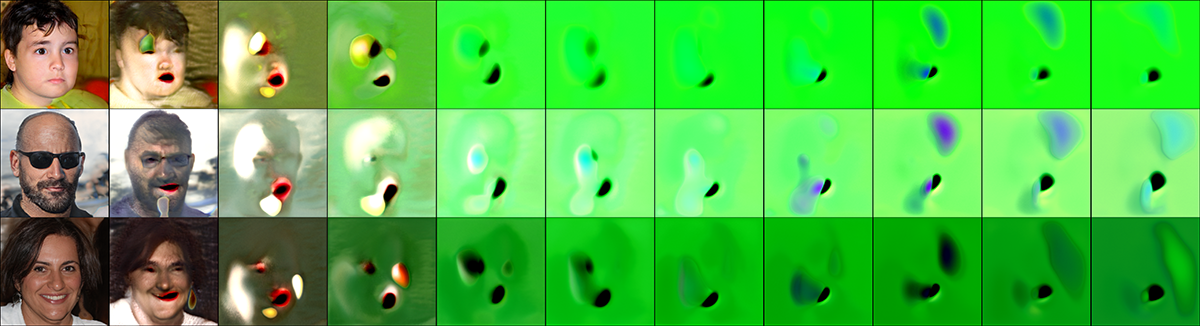
\includegraphics[width=1\textwidth]{figures/c4_divergent/gen-plots/LOG/512/512-LOG-4-Images-10000.png}}
    \hfill
    \subfloat[]{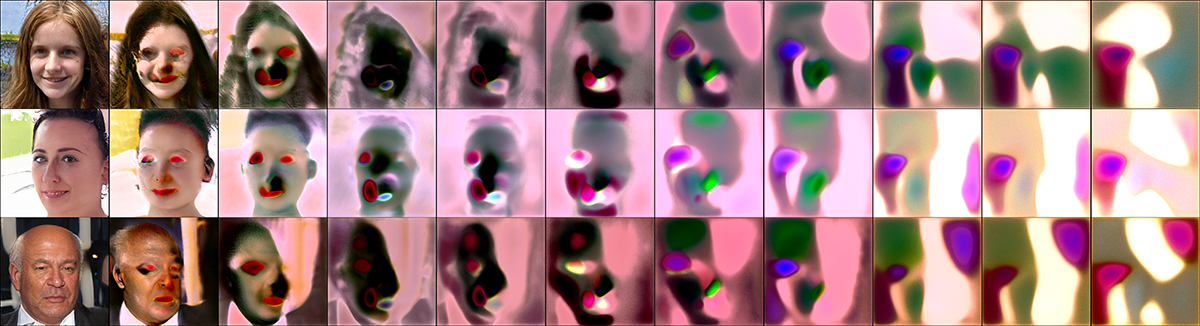
\includegraphics[width=1\textwidth]{figures/c4_divergent/gen-plots/LOG/512/512-LOG-8-Images-10000.png}}
    \caption[Samples of generations during the fine-tuning procedure for 512x512 StyleGAN model with the natural logarithm of the inverted adversarial loss function]{Samples of generations during the fine-tuning procedure for 512x512 StyleGAN model with the natural logarithm of the inverted adversarial loss function, at increments of 1000, between training step 0-10000. (a) Results with batch size 2. (b) Results with batch size 4. (c) Results with batch size 8.}
    \label{fig:c4:512-LOG-samples}
  \end{figure}

  \begin{figure}[!htbp]
    \centering
    \subfloat[]{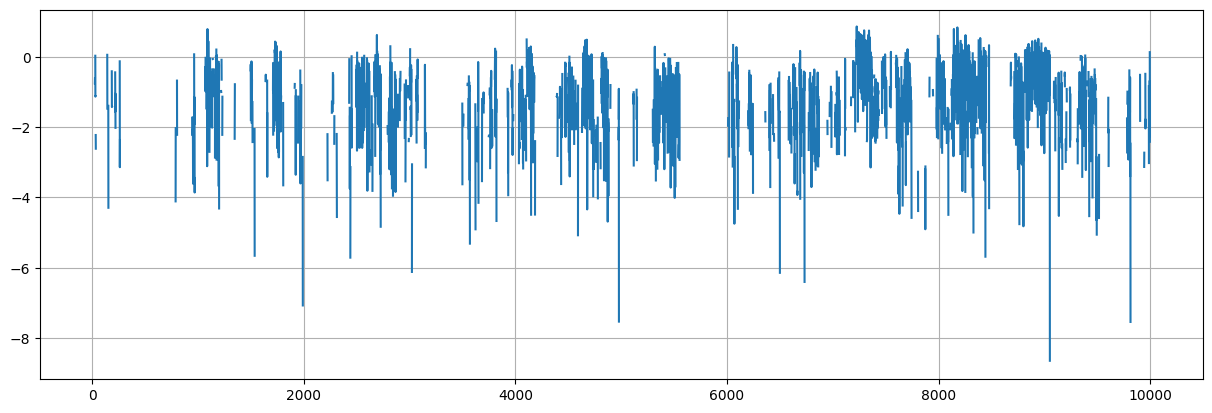
\includegraphics[width=0.8\textwidth]{figures/c4_divergent/loss-plots/LOG/512/512-B2.png}}
    \hfill
    \subfloat[]{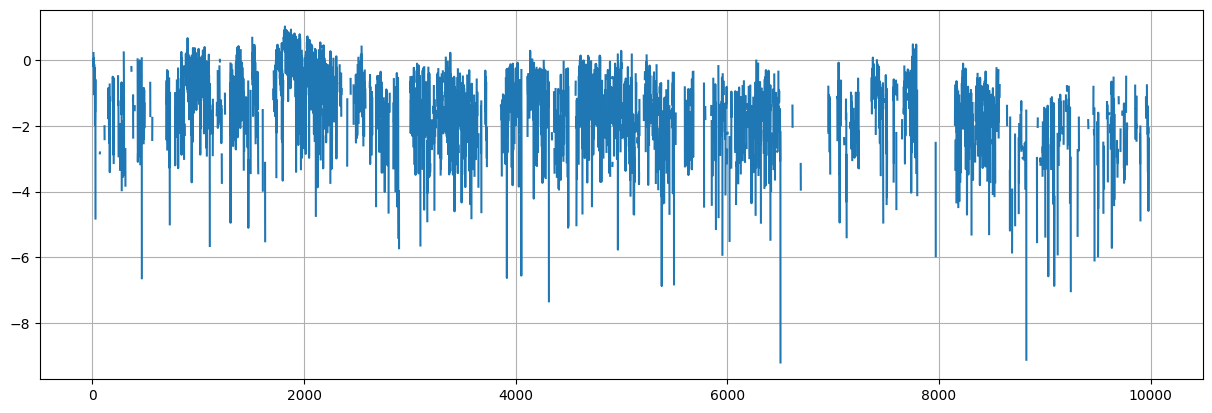
\includegraphics[width=0.8\textwidth]{figures/c4_divergent/loss-plots/LOG/512/512-B4.png}}
    \hfill
    \subfloat[]{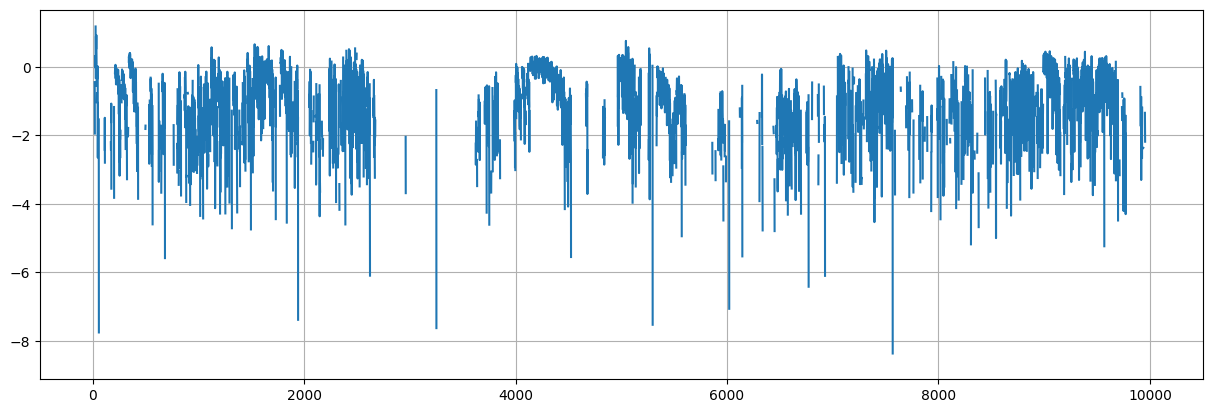
\includegraphics[width=0.8\textwidth]{figures/c4_divergent/loss-plots/LOG/512/512-B8.png}}
    \caption[Loss plots for fine-tuning procedure for 512x512 StyleGAN model with the natural logarithm of the inverted adversarial loss function]{Loss plots for fine-tuning procedure for 512x512 StyleGAN model with the natural logarithm of the inverted adversarial loss function. (a) Results with batch size 2. (b) Results with batch size 4. (c) Results with batch size 8. Note: gaps in the plot are where the loss was undefined from taking the log of a negative number.}
    \label{fig:c4:512-LOG-losses}
  \end{figure}

  \begin{figure}[!htbp]
    \centering
    \subfloat[]{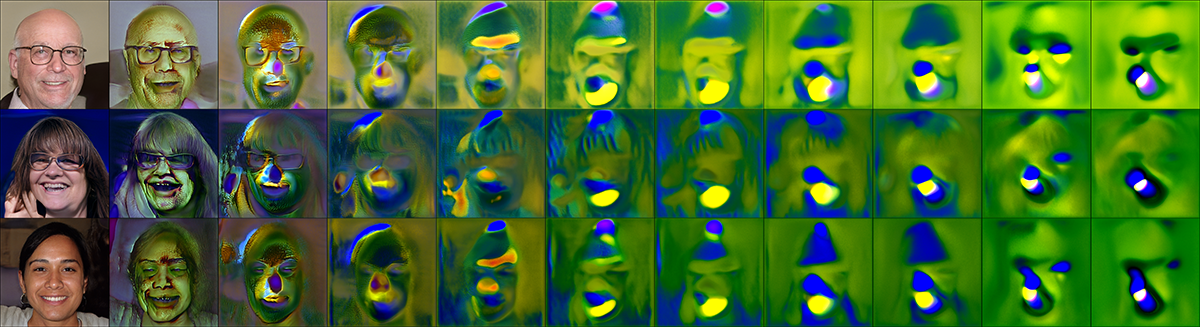
\includegraphics[width=1\textwidth]{figures/c4_divergent/gen-plots/LOG/1024/1024-LOG-2-Images-10000.png}}
    \hfill
    \subfloat[]{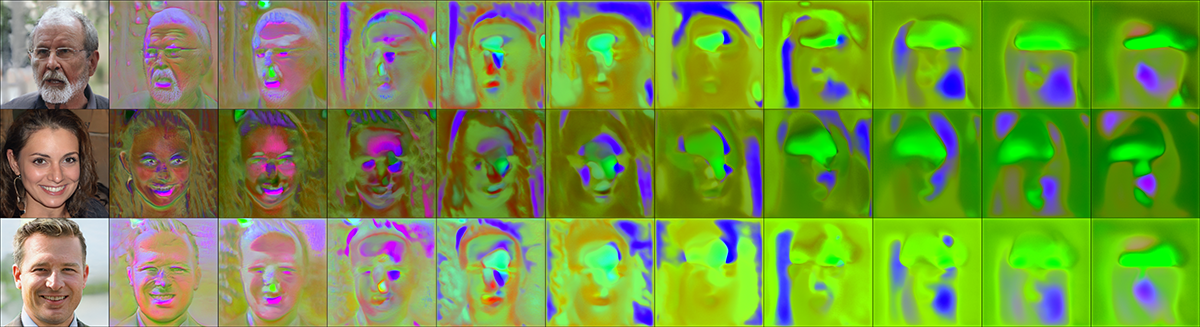
\includegraphics[width=1\textwidth]{figures/c4_divergent/gen-plots/LOG/1024/1024-LOG-4-Images-10000.png}}
    \hfill
    \subfloat[]{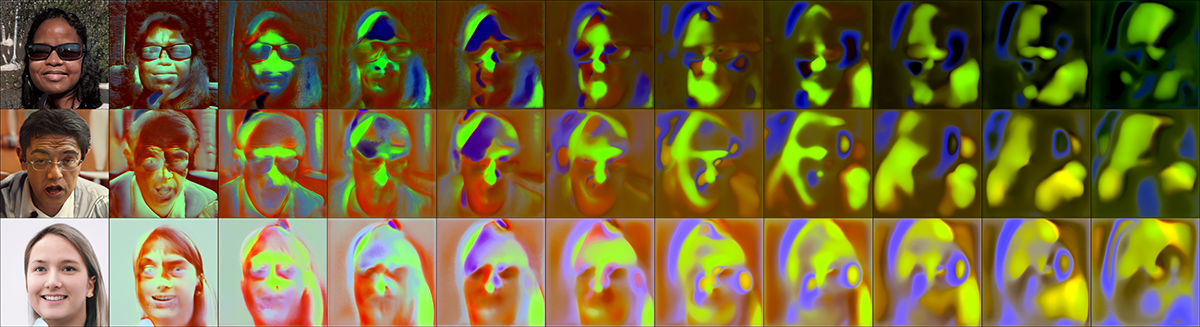
\includegraphics[width=1\textwidth]{figures/c4_divergent/gen-plots/LOG/1024/1024-LOG-8-Images-10000.png}}
    \caption[Samples of generations during the fine-tuning procedure for 1024x1024 StyleGAN model with the natural logarithm of the inverted adversarial loss function]{Samples of generations during the fine-tuning procedure for 1024x1024 StyleGAN model with the natural logarithm of the inverted adversarial loss function, at increments of 1000, between training step 0-10000. (a) Results with batch size 2. (b) Results with batch size 4. (c) Results with batch size 8.}
    \label{fig:c4:1024-LOG-samples}
  \end{figure}

  \begin{figure}[!htbp]
    \centering
    \subfloat[]{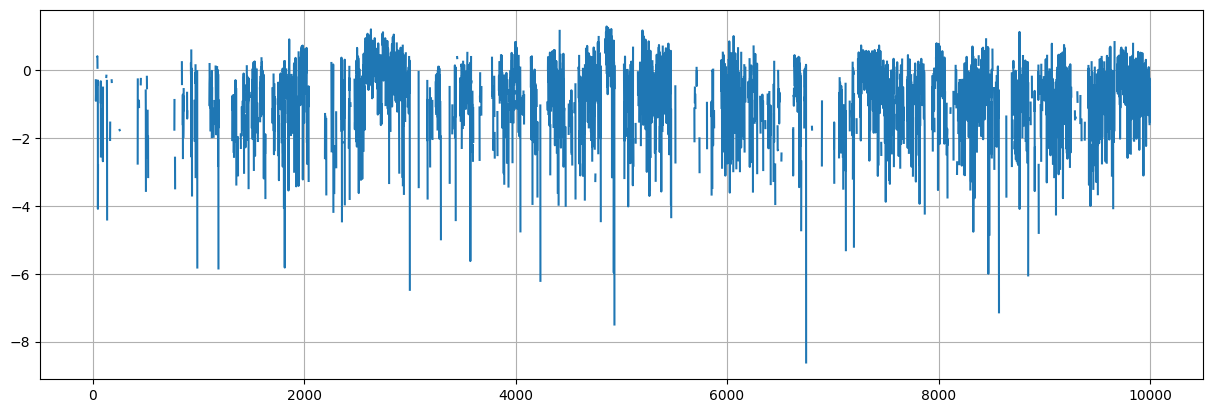
\includegraphics[width=0.8\textwidth]{figures/c4_divergent/loss-plots/LOG/1024/1024-B2.png}}
    \hfill
    \subfloat[]{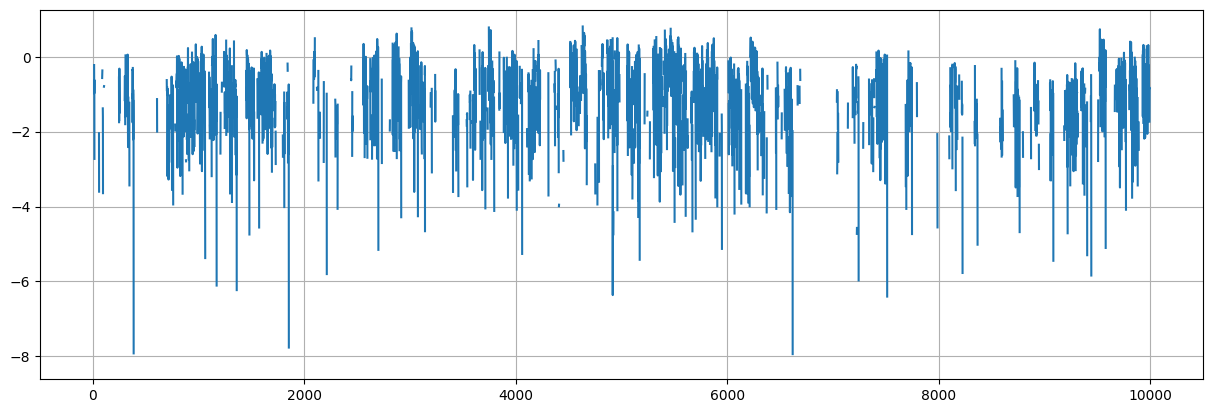
\includegraphics[width=0.8\textwidth]{figures/c4_divergent/loss-plots/LOG/1024/1024-B4.png}}
    \hfill
    \subfloat[]{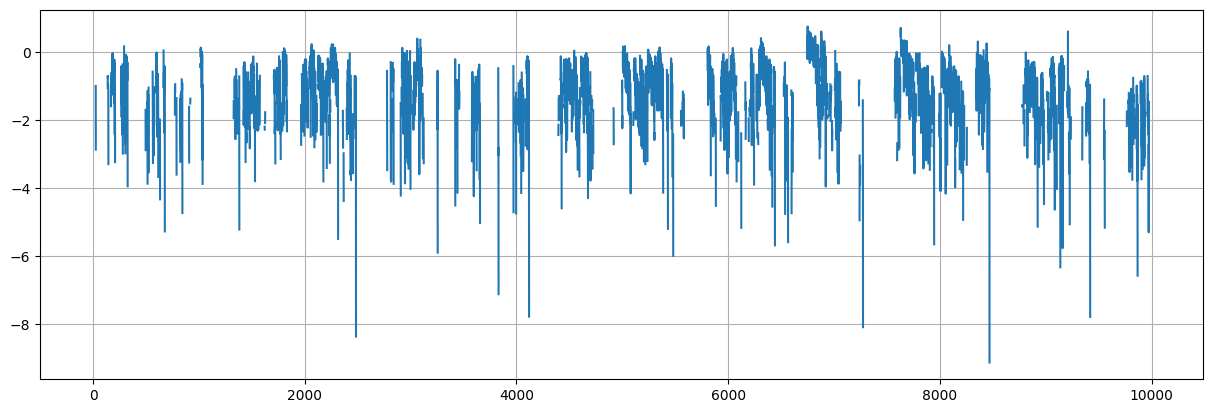
\includegraphics[width=0.8\textwidth]{figures/c4_divergent/loss-plots/LOG/1024/1024-B8.png}}
    \caption[Loss plots for fine-tuning procedure for 1024x1024 StyleGAN model with the natural logarithm of the inverted adversarial loss function]{Loss plots for fine-tuning procedure for 1024x1024 StyleGAN model with the natural logarithm of the inverted adversarial loss function. (a) Results with batch size 2. (b) Results with batch size 4. (c) Results with batch size 8. Note: gaps in the plot are where the loss was undefined from taking the log of a negative number.} 
    \label{fig:c4:1024-LOG-losses}
  \end{figure}

\FloatBarrier

\section{Discussion}

The results presented here demonstrate an efficient method for divergent finetuning that draw the generator away from the likelihood of the original training data (or at least the systems final state). 
The results from the first loss function show a method that quickly optimises towards a fixed representation of `unlikelihood'.
Of course, this representation of unlikelihood is contingent on the particular state of the two models (generator and discriminator) that is then fixed when the model checkpoints are saved during the training process.
GANs, unlike many other training regimes for generative models,  does not converge to a fixed point in the optimisation process.
Instead, they act as a dynamic system, with no target end state. 
The optimisation problem in adversarial approaches is circular \citep{nagarajan2017gradient}. 
The generator and discriminator will forever be playing this game of forger/detective. 
The discriminator endlessly picks up on new minuscule flaws in the generator output, and the generator in turn responds in a potentially eternal adversarial game.
Therefore, for each different saved checkpoint of the discriminator, different attributes that define unlikelihood are being optimised by the generator.
It is clear in the visual results of the different models using the first loss function ( Eq. \ref{eq:inverted-adv-loss}; Figures \ref{fig:c4:256-OG-samples},\ref{fig:c4:512-OG-samples} \& \ref{fig:c4:1024-OG-samples}),that there are specific aspects and features of the image being optimised. 
This shows clearly that this is ever-changing in the training process.

Whilst the results for the standard loss show that there is a generally coherent fixed point of optimisation for each of the model snapshots, there are minor visual differences in each of the different training runs.
Whilst it would be easy to attribute this solely to the change in the batch size parameter, I suspect that the sampling regime is also a contingent part of the visual differences between the training runs.
Input latents for the generator are sampled randomly, and this random sampling and the sequence in which random latents are sampled may be just as important in determining the direction for optimisation and the final visual results, as much as the batch size used in each of these training runs. 

For the second loss function \ref{eq:ln-inverted-adv-loss}, which uses the natural log of the inverse adversarial loss, there is clearly much less of a fixed point to which the optimiser is moving. 
Whilst there are similarities in all of these final results (abstract shapes with generally consistent colours), there is clearly not one fixed point here that is being optimised for each of the model checkpoints.
Taking the log of the loss appears to constrain the loss function better.
The logs of the losses with the standard adversarial loss (Eq. \ref{eq:inverted-adv-loss}) quickly explode into very high ranges (exceeding -600000 in some cases).
This is due to the feedback loop of reinforcing changes, where any change to the parameters of the generator further increases the loss.
By taking the log of the loss this feedback loop is nullified. 
There are likely two things at play here.
In log space the exponential feedback loop is far less aggressive. 
As these loss scores also tend towards negative numbers, when we take the log of this loss, these negative numbers become undefined (as taking the log of a negative number is always undefined).
As you can see in Figures \ref{fig:c4:256-LOG-losses},\ref{fig:c4:512-LOG-losses} \& \ref{fig:c4:1024-LOG-losses}, there are large gaps where there is loss in underfined.\footnote{Surprisingly, backpropagating undefined numbers does not seem to be an issue in pytorch.}
Once again this may act as a constraint that prevents the feedback loop seen in Figures \ref{fig:c4:256-OG-losses},\ref{fig:c4:512-OG-losses} \& \ref{fig:c4:1024-OG-losses} from taking hold.

The fine-tuning procedure using Eq. \ref{eq:ln-inverted-adv-loss} appears to produce a dynamic between models between models that may be endless. 
Figure \ref{fig:c4:100k-iterations} shows one of these training runs continuing to 100,000 iterations,where it appears this process is still evolving.
Similarly to the work in Chapter \ref{ch:unstable_eq} this is an endless and undefined goal, leading to a dynamic process that continually produces ever-evolving abstract outputs.

\begin{figure}[!htbp]
  \centering
  \subfloat[]{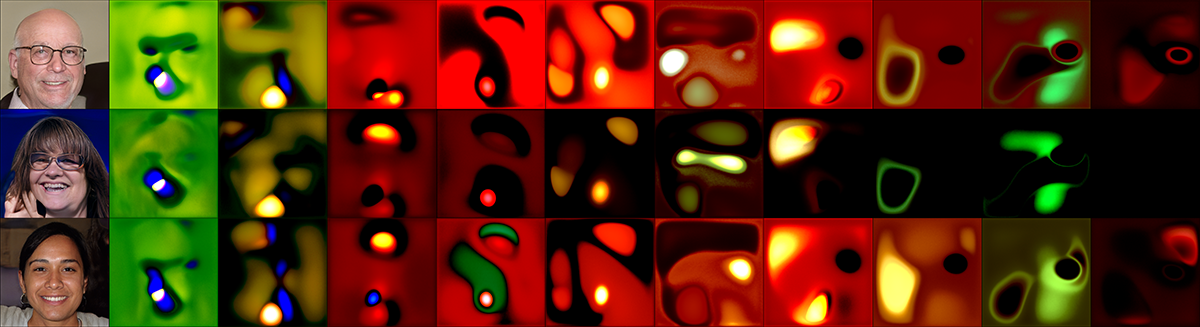
\includegraphics[width=1\textwidth]{figures/c4_divergent/discussion/log-8-100k-iterations.png}}
  \caption[100k iterations of 1024x1024 StyleGAN model with the natural logarithm of the inverted adversarial loss function]{100k iterations of 1024x1024 StyleGAN model with the natural logarithm of the inverted adversarial loss function with batch parameter 8, at increments of 10000, between training step 0-100000.}
  \label{fig:c4:100k-iterations}
\end{figure}

\subsection{Relationship to The Uncanny}

One of the observations that was made regarding the visual results of this process, especially in the transition stages of standard inverted loss, was the uncanny nature of the images,\footnote{
      Some of the early images I created during this process were quite disturbing  (Ref impact chapter). The first person I showed them to was my partner at the time, whose response was to the effect of: ``Well that is horrifying, please never show me those pictures again''. I later showed the results to a PhD colleague of mine, Shringi Kumari, in the Goldsmiths iGGi office, who had an equally negative reaction.} which can be seen in Figures \ref{fig:c4:uncanny-images-og} \& \ref{fig:c4:uncanny-images-log}.

\begin{figure}[!htbp]
  \vspace{-60pt}
  \centering
  \subfloat[]{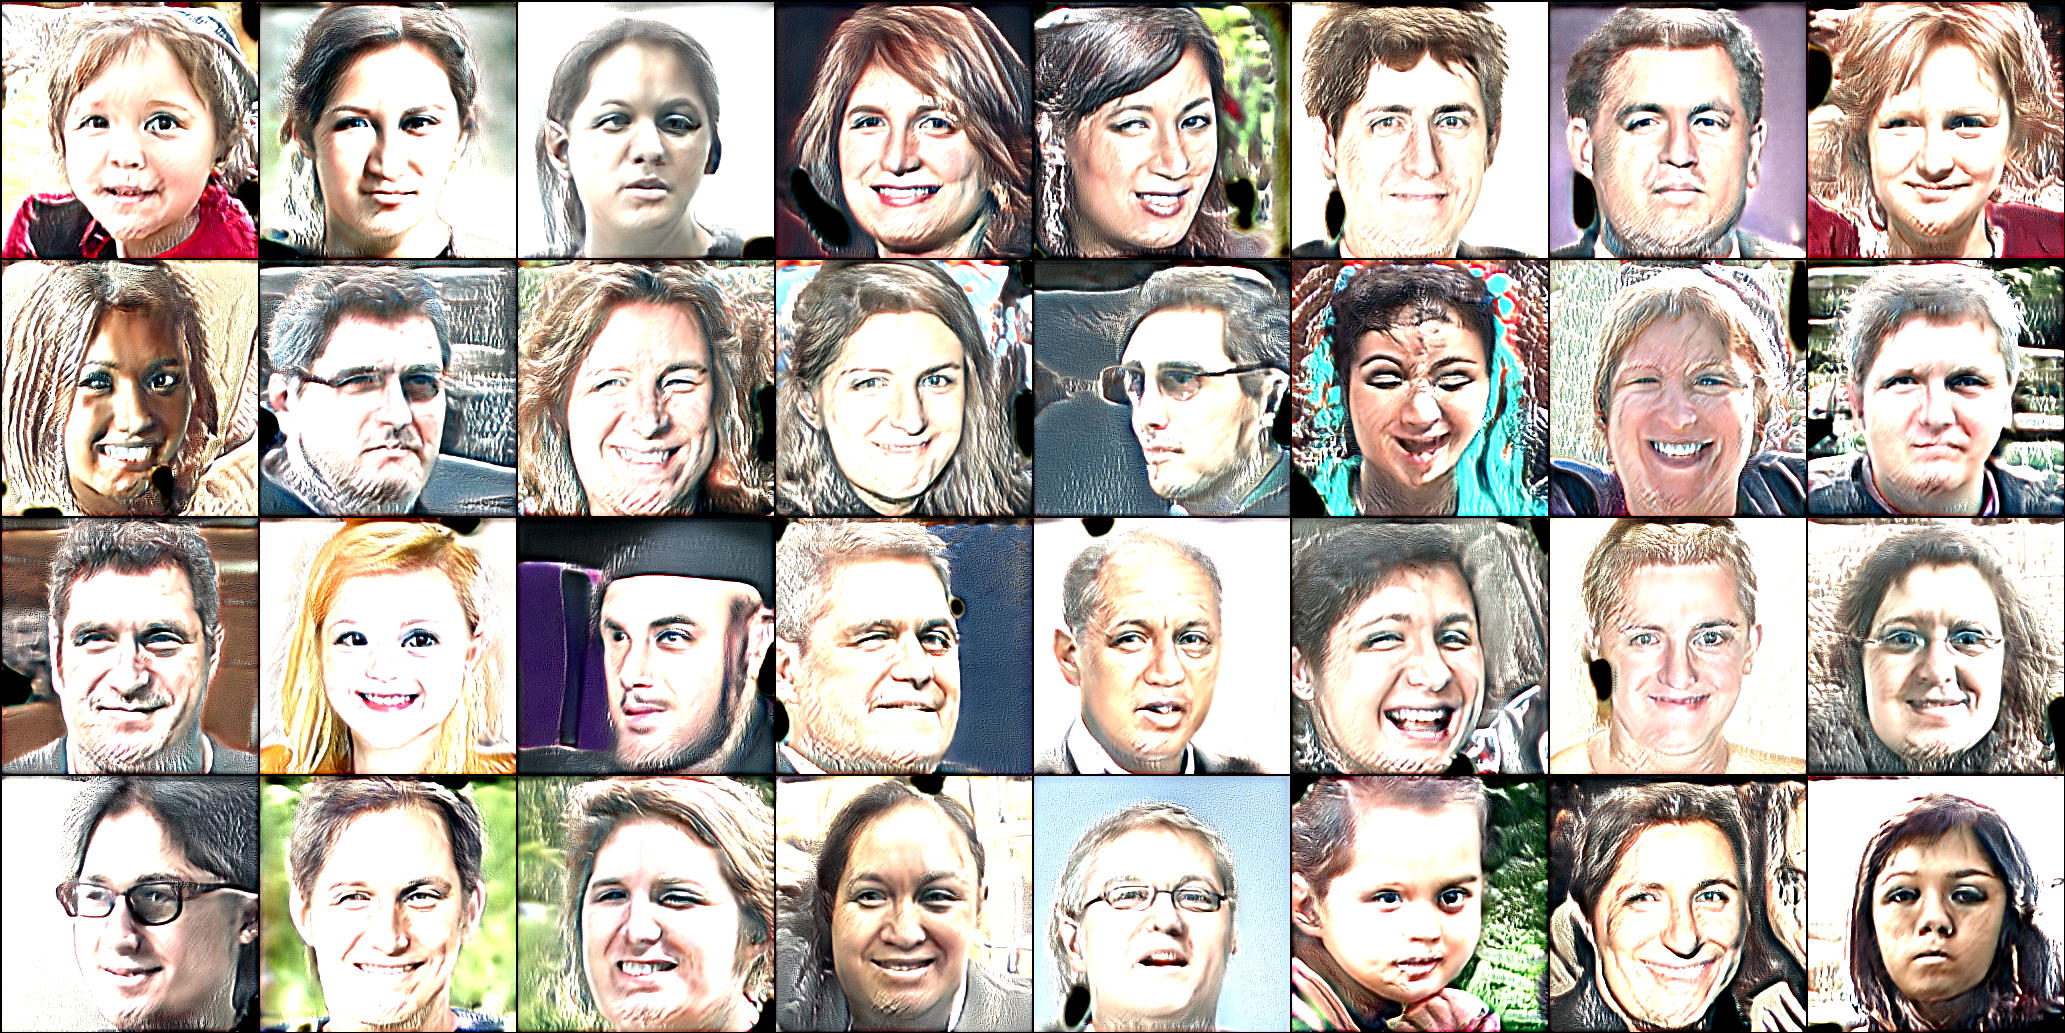
\includegraphics[width=1\textwidth]{figures/c4_divergent/discussion/grid-256-300iter.png}}
  \hfill
  \subfloat[]{\includegraphics[width=1\textwidth]{figures/c4_divergent/discussion/grid-512-300iter.png}}
  \hfill
  \subfloat[]{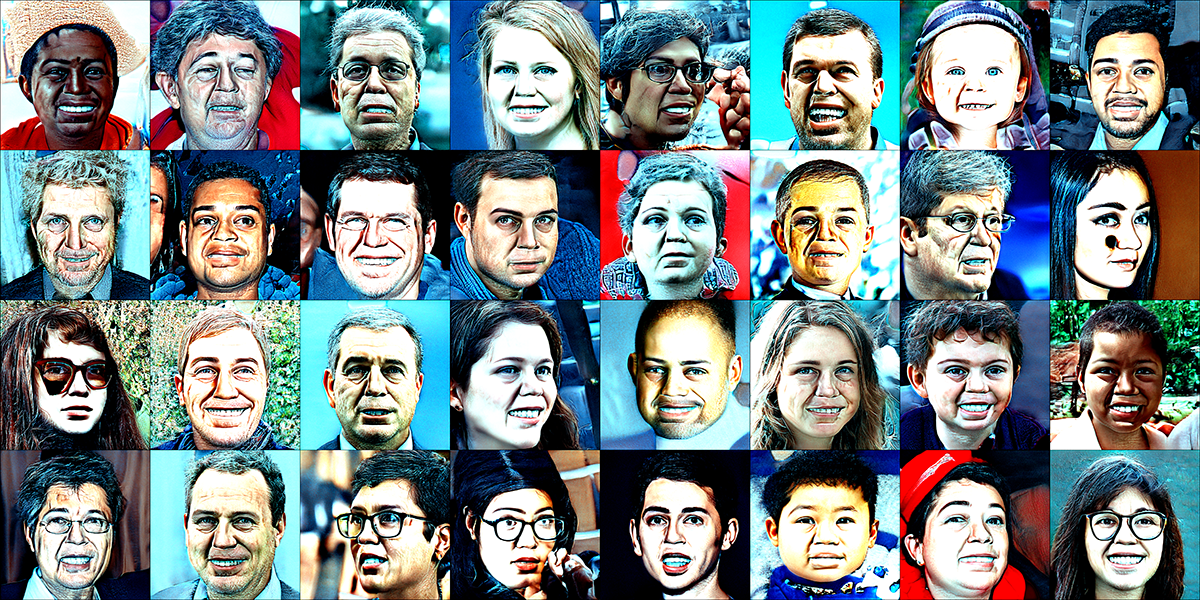
\includegraphics[width=1\textwidth]{figures/c4_divergent/discussion/grid-1024-300iter.png}}
  \caption[Uncanny images of samples from 300 iterations of fine-tuning with inverse loss]{Uncanny images of samples from 300 iterations of fine-tuning with inverse loss, using batch size of 2. (a) 256x256 model. (b) 512x512 model. (c) 1024x1024 model. }
  \label{fig:c4:uncanny-images-og}
\end{figure}

\begin{figure}[!htbp]
  \vspace{-60pt}
  \centering
  \subfloat[]{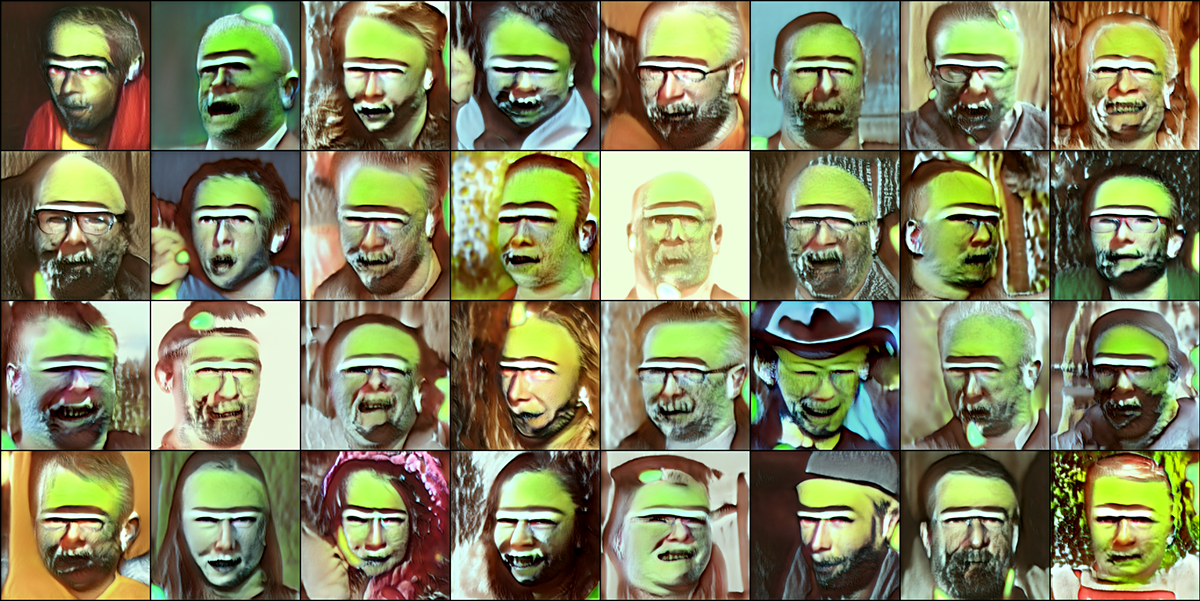
\includegraphics[width=1\textwidth]{figures/c4_divergent/discussion/grid-256-1000iter-log.png}}
  \hfill
  \subfloat[]{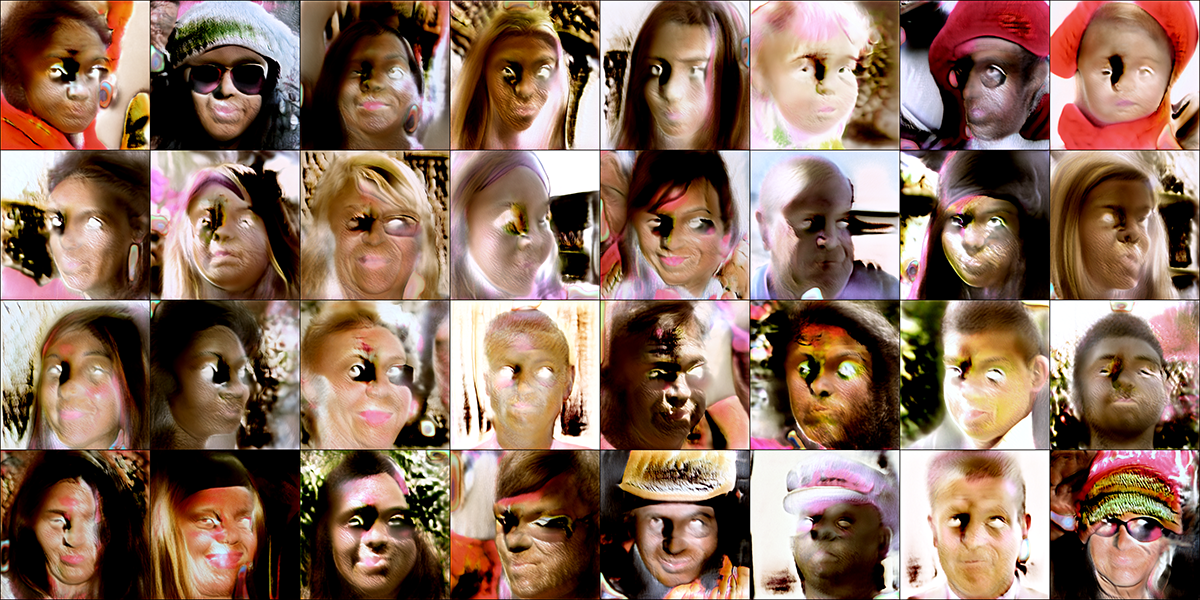
\includegraphics[width=1\textwidth]{figures/c4_divergent/discussion/grid-512-1000iter-log.png}}
  \hfill
  \subfloat[]{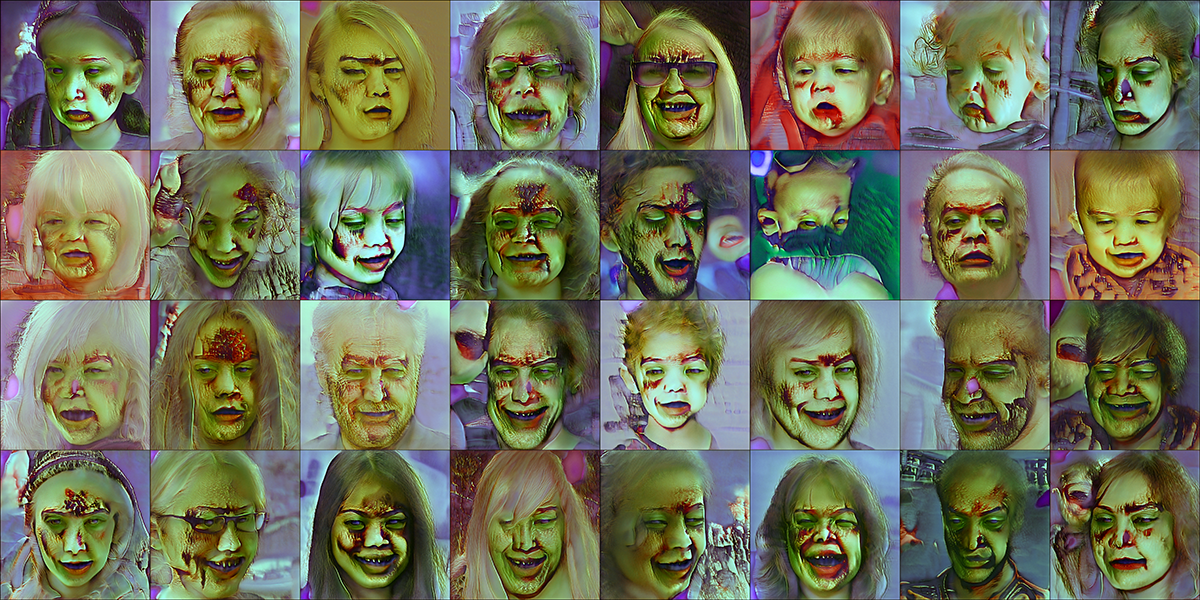
\includegraphics[width=1\textwidth]{figures/c4_divergent/discussion/grid-1024-1000iter-log.png}}
  \caption[Uncanny images of samples from 1000 iterations of fine-tuning with natural logarithm of the inverse loss]{Uncanny images of samples from 1000 iterations of fine-tuning with natural logarithm of the inverse loss, using batch size of 2. (a) 256x256 model. (b) 512x512 model. (c) 1024x1024 model. }
  \label{fig:c4:uncanny-images-log}
\end{figure}

The uncanny is a psychological or aesthetic experience that can be characterised as observing something familiar that is encountered in an unsettling way. 
Jentsch defined the uncanny as an experience that stems from uncertainty, giving an example of it as being most pronounced when there is “doubt as to whether an apparently living being is animate and, conversely, doubt as to whether a lifeless object may not in fact be animate” \citep{jentsch1906psychology}. 
This definition was later refined to argue that the uncanny occurs when something familiar is alienated when the familiar is viewed in an unexpected or unfamiliar form \citep{freud1919uncanny}.

The uncanny valley is a concept first introduced in 1970 by Masahiro Mori, a professor of robotics. 
It describes how in the field of robotics,, an increase in the fidelity of human likeness increases feelings of familiarity up to a point (Figure \ref{subfig:uncanny-valley}), before suddenly decreasing. 
As representations of human or animal likeness approach a close resemblance to human or animal form, it provokes an unsettling feeling. 
Responses in likeness and familiarity rapidly become more negative than at any prior point. 
It is only when the robotic form is close to imperceptible with respect to human or animal likeness that the familiarity response becomes positive again \citep{mori1970uncanny}. 
As well as in robotics, this phenomenon has been observed in video games \citep{ratajczyk2019uncanny}, visual effects \citep{schwind2018avoiding}, and animation \citep{assaf2020presence}.

In visual arts, the uncanny can be used deliberately to evoke unsettling feelings and explore boundaries between what is living and what is machine. This often reflects the anxieties and technologies of any given era, such as interactive robotic installations in the late 20th Century \citep{tronstad2008uncanny}. 
In work from the early 20th Century, such as Jacob Epsteins \textit{Rock Drill} (circa 1913) which depicts the human form as transformed and amalgamated by industrial machinery \citep{grenville2001uncanny}. 
In the moving image, Czech animator Jan Svankmajer is well known for creating animated representations of the human form that deliberately confuse the viewer with respect to notions of life and lifelessness \citep{chryssouli2019alchemist}.

The process of fine-tuning shown in \S \ref{c4:sec:results} can be described as crossing the uncanny valley in reverse (Figure \ref{fig:c4:uncanny-valley-comparison}).
The original StyleGAN model trained on FFHQ was one of the first generative models to be able to generate images that were completely indistinguishable from real people to the untrained eye \citep{ajder2019state}, and a sophisticated understanding of the flaws of these models is needed in order to spot these deepfakes \citep{mcdonald2018how}. 
Given the fact that images from these models have been used to make fake social media accounts \citep{satter2019spy} by spies trying to penetrate the American defence establishment, it is clear that StyleGAN-generated images, at least in some instances, have crossed the threshold of the uncanny valley towards producing completely plausible and convincing images of people.
Starting from realism, and training towards abstraction, the process crosses the uncanny valley in reverse. 
As the generator starts to diverge from realism the images quickly become increasingly unsettling, before starting to plateau back to abstraction and returning to a more favourable likeness.

\begin{figure}[!htbp]
  \centering
  \subfloat[]{\label{subfig:uncanny-valley}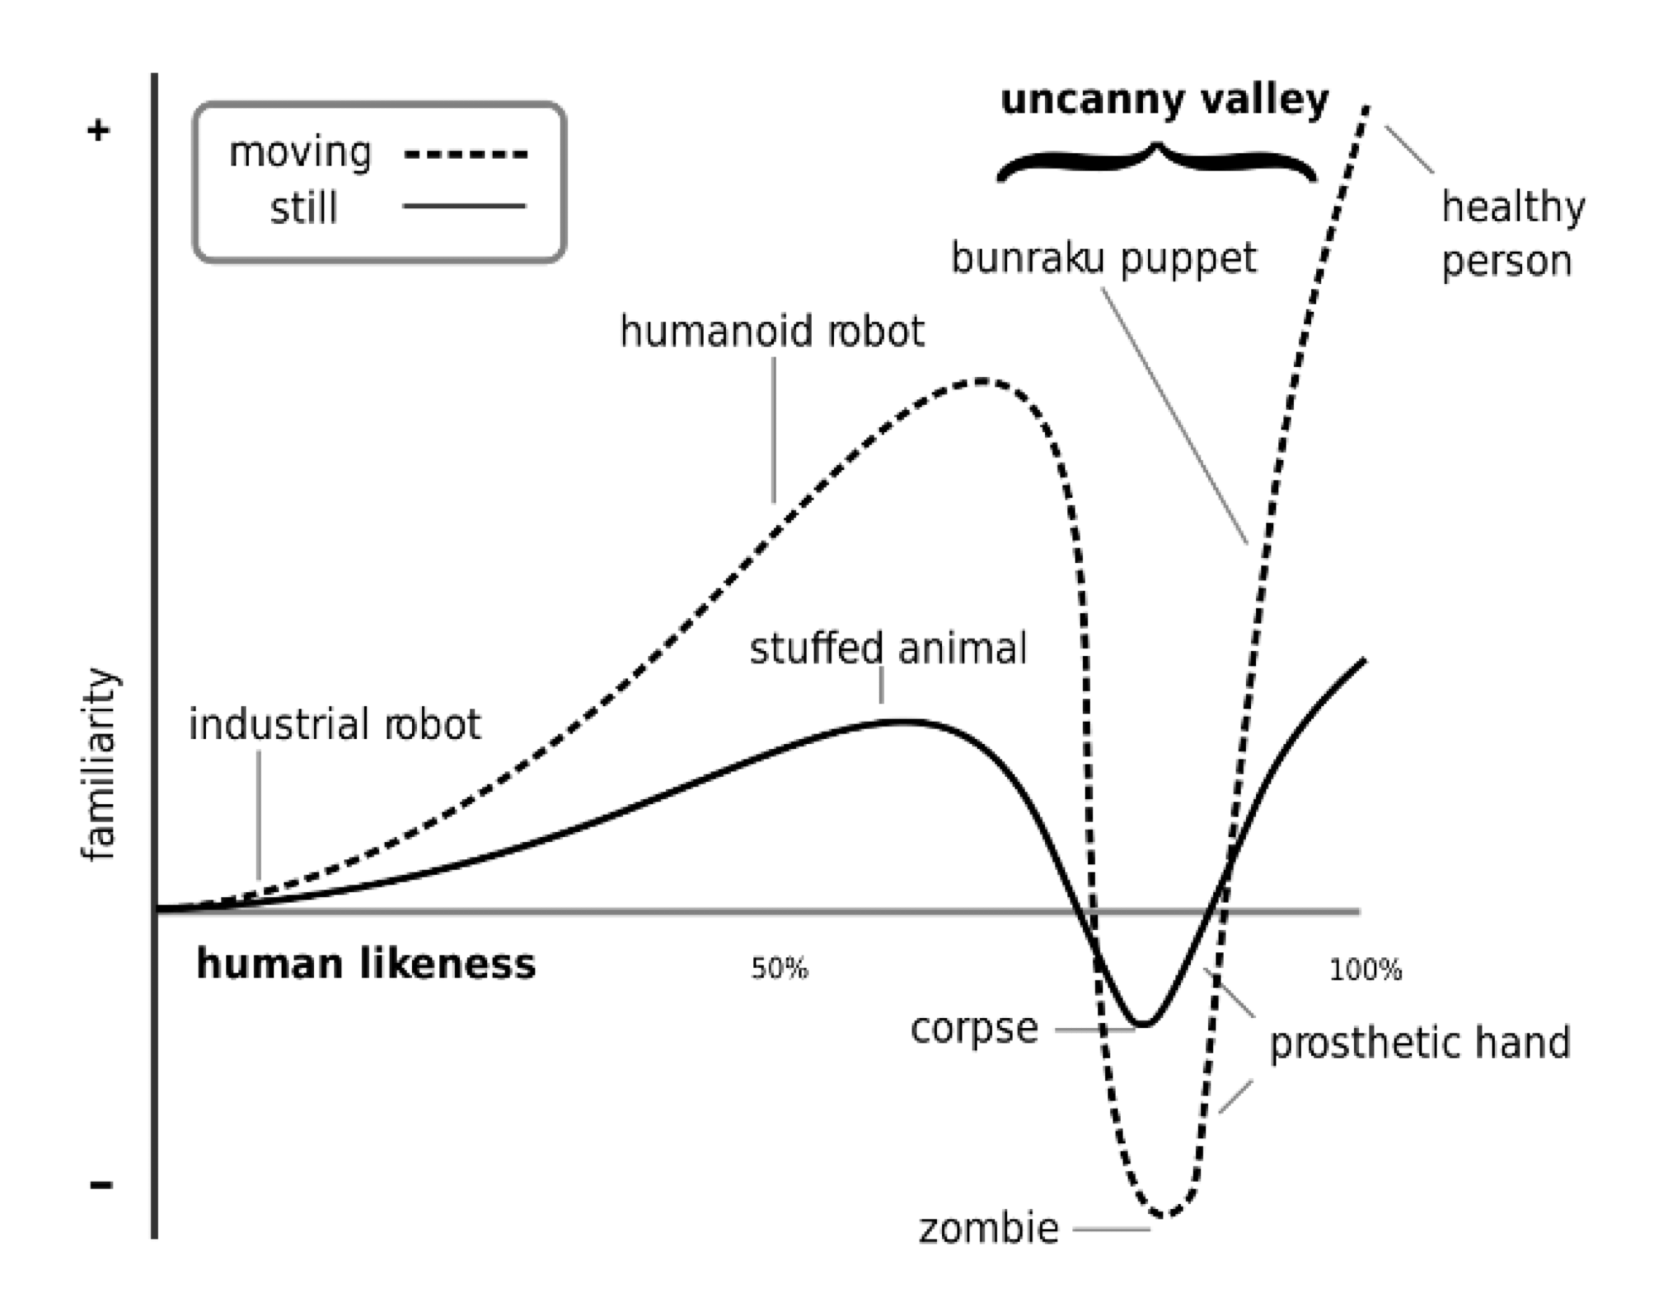
\includegraphics[width=1\textwidth]{figures/c4_divergent/diagrams/uncanny-valley.png}}
  \hfill
  \subfloat[]{\label{subfig:reversed-fine-tune}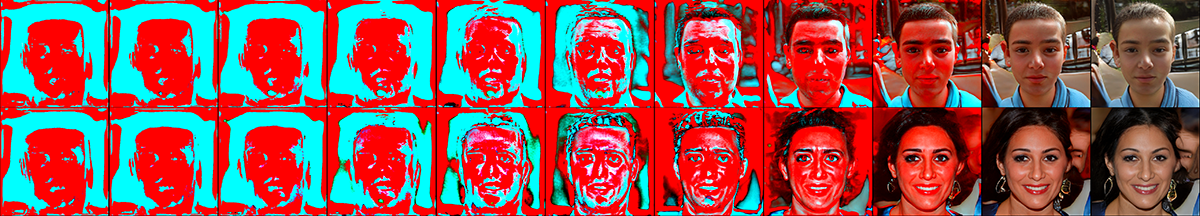
\includegraphics[width=1\textwidth]{figures/c4_divergent/diagrams/uncanny-valley-reverse-512-OG-B8.png}}
  \caption[Uncanny valley diagram juxtaposed with samples from fine-tuning process]{Uncanny valley diagram juxtaposed with fine-tuning samples in reverse order. (a) Diagram showing the uncanny valley \citep{mori1970uncanny}. (b) Samples from the fine-tuning procedure in Figure \ref{fig:c4:512-OG-samples} (512x512 finetuned with loss \ref{eq:inverted-adv-loss} with batch parameter 8) in reverse order. Diagram (a) reproduced under a CC BY-SA 3.0 licence. }
  \label{fig:c4:uncanny-valley-comparison}
\end{figure}

\section{Conclusion}

In this chapter, I have demonstrated an approach to fine-tuning pre-trained generative neural networks in a data-divergent fashion that does not rely on imitation-based learning.
This approach was the first peer-reviewed and published method for divergent finetuning (to the best of my knowledge).
A complete account of other known methods for divergent finetuning to date is given in \S \ref{survey:divergent}.

While this work is novel, the results from all of the training runs described here are very idiosyncratic. 
The results are contingent on the unique state that the auxiliary models are in when their parameters are saved into checkpoints during training. 
In the case of the discriminator, this is completely unpredictable and not repeatable. 
While this can make for surprising outcomes, it also means that the experiments described would be impossible to reproduce without the exact model checkpoints (and sequence of latent that are sampled in fine-tuning).

How would it be possible then to manipulate a generative network in a way that was more controllable and repeatable?
This became a question that was playing on my mind after doing these experiments. 
The techniques described here use gradient descent to manipulate the weights of the model to produce novel outcomes. 
The process of gradient descent, however, is not something that we as humans can clearly understand, or easily control.
I became preoccupied with finding a way of manipulating generative models, without relying on gradient descent. 
The next chapter is the third and final chapter that details a novel technical contribution of in this thesis, one that centres humans in the creative process and allows them to manipulate generative neural networks without training of fine-tuning whatsoever.
